 \documentclass[empirical, authordate]{jote-new-article}

\begin{filecontents}{bibliography.bib}
@article{Hunt2003,
  author = {Hunt, Nicholas H and Grau, G E },
  date = {2003},
  title = {Cytokines: accelerators and brakes in the pathogenesis of cerebral malaria},
  volume = {24},
  pages = {491-499},
  url = {https://doi.org/10.1016/S1471-4906(03)00229-1},
  doi = {10.1016/S1471-4906(03)00229-1},
  language = {en},
  journal = {Trends in Immunology},
  number = {9}
}
@misc{DeSouza2010,
  author = {De Souza, J  and Hafalla, J C R  and Riley, E M  and Couper, K N },
  date = {2010},
  title = {Cerebral malaria: Why experimental murine models are required to understand the pathogenesis of disease},
  url = {https://doi.org/10.1017/S0031182009991715},
  doi = {10.1017/S0031182009991715},
  language = {es},
  type = {Parasitology.}
}
@article{Lou2001,
  author = {Lou, J  and Lucas, R  and Grau, G E },
  date = {2001},
  title = {Pathogenesis of Cerebral Malaria},
  volume = {14},
  pages = {810-820},
  url = {https://doi.org/10.1128/CMR.14.4.810},
  doi = {10.1128/CMR.14.4.810},
  language = {en},
  journal = {Recent Experimental Data and Possible Applications for Humans},
  number = {4}
}

  @article{Hunt2006,
    title       = {Immunopathogenesis of cerebral malaria},
    author      = {Hunt, Nicholas H and Golenser, Jacob and Chan-Ling, Tailoi and Parekh, Sapan and Rae, Caroline and Potter, Sarah and Medana, Isabelle M and Miu, Jenny and Ball, Helen J},
    number      = {5},
    volume      = {36},
    doi         = {10.1016/J.IJPARA.2006.02.016},
    publisher   = {Pergamon},
    year        = {2006},
    pages       = {569-582},
    journal     = {International Journal for Parasitology}
}


@article{Bartoloni2012,
    title       = {Clinical aspects of uncomplicated and severe malaria.},
    author      = {Bartoloni, Alessandro and Zammarchi, Lorenzo},
    number      = {1},
    volume      = {4},
    doi         = {10.4084/MJHID.2012.026},
    publisher   = {Catholic University in Rome},
    year        = {2012},
    pages       = {e2012026},
    journal     = {Mediterranean journal of hematology and infectious diseases}
}


@article{Grau1987,
    title       = {Tumor necrosis factor (cachetin) as an essential mediator in murine cerebral malaria},
    author      = {Grau, Georges E and Fajardo, Luis F and Piguet, Pierre-Francois and Allet, Bernard and Lambert, Paul-Henri and Vassalli, Pierre},
    number      = {4819},
    volume      = {237},
    year        = {1987},
    pages       = {1210-1213},
    journal     = {Science}
}


@article{Medana2006,
    title       = {Human cerebral malaria and the blood--brain barrier},
    author      = {Medana, Isabelle M and Turner, Gareth D H},
    number      = {5},
    volume      = {36},
    doi         = {10.1016/J.IJPARA.2006.02.004},
    publisher   = {Pergamon},
    year        = {2006},
    pages       = {555-568},
    journal     = {International Journal for Parasitology}
}


@article{Linares2013,
    title       = {Brain-derived neurotrophic factor and the course of experimental cerebral malaria},
    author      = {Linares, María and Marín-García, Patricia and Pérez-Benavente, Susana and Sánchez-Nogueiro, Jesús and Puyet, Antonio and Bautista, José M and Diez, Amalia},
    volume      = {1490},
    doi         = {10.1016/j.brainres.2012.10.040},
    year        = {2013},
    pages       = {210-224},
    journal     = {Brain Research}
}


@article{Mariotti2011,
    title       = {Neuroinflammation and brain infections: Historical context and current perspectives},
    author      = {Mariotti, Raffaella and Bertini, Giuseppe},
    number      = {1-2},
    volume      = {66},
    doi         = {10.1016/J.BRAINRESREV.2010.09.008},
    publisher   = {Elsevier},
    year        = {2011},
    pages       = {152-173},
    journal     = {Brain Research Reviews}
}


@article{Combes2006,
    title       = {Cerebral malaria: role of microparticles and platelets in alterations of the blood-brain barrier},
    author      = {Combes, Valéry and Coltel, Nicolas and Faille, Dorothée and Wassmer, Samuel Crocodile and Grau, Georges Emile},
    number      = {5},
    volume      = {36},
    doi         = {10.1016/j.ijpara.2006.02.005},
    year        = {2006},
    pages       = {541-546},
    journal     = {International Journal for Parasitology}
}


@article{Fogaça2013,
    title       = {Cannabinoids, Neurogenesis and Antidepressant Drugs: Is there a Link?},
    author      = {Fogaça, Manoela Viar and Galve-Roperh, Ismael and Guimarães, Francisco Silveira and Campos, Alline Cristina},
    number      = {3},
    volume      = {11},
    doi         = {10.2174/1570159X11311030003},
    publisher   = {Bentham Science Publishers},
    year        = {2013},
    pages       = {263-275},
    journal     = {Current neuropharmacology}
}


@article{Fernández-Ruiz2015,
    title       = {Endocannabinoids and neurodegenerative disorders: Parkinson's disease, huntington's chorea, alzheimer's disease, and others},
    author      = {Fernández-Ruiz, Javier and Romero, Julián and Ramos, José A},
    volume      = {231},
    doi         = {10.1007/978-3-319-20825-1\_8},
    year        = {2015},
    pages       = {233-259},
    journal     = {Endocannabinoids}
}


@article{Pazos2012,
    title       = {Cannabidiol administration after hypoxia--ischemia to newborn rats reduces long-term brain injury and restores neurobehavioral function},
    author      = {Pazos, M R and Cinquina, V and Gómez, A and Layunta, R and Santos, M and Fernández-Ruiz, J and Martínez-Orgado, José},
    number      = {5},
    volume      = {63},
    doi         = {10.1016/j.neuropharm.2012.05.034},
    year        = {2012},
    pages       = {776-783},
    journal     = {Neuropharmacology}
}


@article{Alferink2016,
    title       = {Cannabinoid receptor 2 modulates susceptibility to experimental cerebral malaria through a CCL17-dependent Mechanism},
    author      = {Alferink, Judith and Specht, Sabine and Arends, Hannah and Schumak, Beatrix and Schmidt, Kim and Ruland, Christina and Lundt, Ramona and Kemter, Andrea and Dlugos, Andrea and Kuepper, Janina M and Poppensieker, Karola and Findeiss, Matthias and Albayram, Nder and Otte, David M and Marazzi, Janine and Gertsch, Jürg and Förster, Irmgard and Maier, Wolfgang and Scheu, Stefanie and Hoerauf, Achim and Zimmer, Andreas},
    number      = {37},
    volume      = {291},
    doi         = {10.1074/jbc.M116.746594},
    year        = {2016},
    pages       = {19517-19531},
    journal     = {Journal of Biological Chemistry}
}


@article{Campos2015,
    title       = {Cannabidiol increases survival and promotes rescue of cognitive function in a murine model of cerebral malaria},
    author      = {Campos, A C and Brant, F and Miranda, A S and Machado, F S and Teixeira, A L},
    volume      = {289},
    doi         = {10.1016/j.neuroscience.2014.12.051},
    year        = {2015},
    pages       = {166-180},
    journal     = {Neuroscience}
}


@article{Martínez-Pinilla2017,
    title       = {Binding and Signaling Studies Disclose a Potential Allosteric Site for Cannabidiol in Cannabinoid CB 2 Receptors},
    author      = {Martínez-Pinilla, Eva and Varani, Katia and Reyes-resina, Irene and Angelats, Edgar and Vincenzi, Fabrizio and Ferreiro-vera, Carlos and Oyarzabal, Julen and Canela, Enric I and Lanciego, José L and Nadal, Xavier and Navarro, Gemma and Borea, Pier Andrea and Franco, Rafael and Lane, J Robert David},
    number      = {October},
    journal     = {Frontiers in Pharmacology},
    volume      = {8},
    doi         = {10.3389/fphar.2017.00744},
    year        = {2017},
    pages       = {1-10}
}


@article{Portier1999,
    title       = {SR 144528, an antagonist for the peripheral cannabinoid receptor that behaves as an inverse agonist - PubMed},
    author      = {Portier, M and Rinaldi-Carmona, M and Pecceu, F and Combes, T and Poinoit-Chazel, C and Calandra, B and Barth, F and Le Fur, G and Casellas, P},
    number      = {2},
    volume      = {288},
    year        = {1999},
    pages       = {582-589},
    journal     = {Journal of Pharmacology and Experimental Therapeutics}
}


@article{Rinaldi-Carmona1998,
    title       = {SR 144528, the first potent and selective antagonist of the CB2 cannabinoid receptor},
    author      = {Rinaldi-Carmona, Murielle and Barth, Francis and Millan, José and Derocq, Jean Marie and Casellas, Pierre and Congy, Christian and Oustric, Didier and Sarran, Martine and Bouaboula, Monsif and Calandra, Bernard and Portier, Marielle and Shire, David and Brelière, Jean Claude and Le Fur, Gérard},
    number      = {2},
    volume      = {284},
    publisher   = {American Society for Pharmacology and Experimental Therapy},
    year        = {1998},
    pages       = {644-650},
    journal     = {Journal of Pharmacology and Experimental Therapeutics}
}


@article{Rinaldi-Carmona1994,
    title       = {SR141716A, a potent and selective antagonist of the brain cannabinoid receptor},
    author      = {Rinaldi-Carmona, Murielle and Barth, Francis and Héaulme, Michel and Shire, David and Calandra, Bernard and Congy, Christian and Martinez, Serge and Maruani, Jeanne and Néliat, Gervais and Caput, Daniel and Ferrara, Pascual and Soubrié, Philippe and Brelière, Jean Claude and Le Fur, Gérard},
    number      = {2-3},
    volume      = {350},
    doi         = {10.1016/0014-5793(94)00773-X},
    publisher   = {FEBS Lett},
    year        = {1994},
    pages       = {240-244},
    journal     = {FEBS letters}
}


@article{Cumella2012,
    title       = {Chromenopyrazoles: Non-psychoactive and Selective CB 1 Cannabinoid Agonists with Peripheral Antinociceptive Properties},
    author      = {Cumella, Jose and Hernández-Folgado, Laura and Girón, Rocio and Sánchez, Eva and Morales, Paula and Hurst, Dow P and Gómez-Cañas, Maria and Gómez-Ruiz, Maria and Pinto, Diana C G A and Goya, Pilar and Reggio, Patricia H and Martin, María Isabel and Fernández-Ruiz, Javier and Silva, Artur M S and Jagerovic, Nadine},
    number      = {3},
    volume      = {7},
    doi         = {10.1002/cmdc.201100568},
    year        = {2012},
    pages       = {452-463},
    journal     = {ChemMedChem}
}


@article{Deiana2016,
    title       = {Tricyclic pyrazoles. Part 8. Synthesis, biological evaluation and modelling of tricyclic pyrazole carboxamides as potential CB2 receptor ligands with antagonist/inverse agonist properties},
    author      = {Deiana, Valeria and Gómez-Cañas, María and Pazos, M Ruth and Fernández-Ruiz, Javier and Asproni, Battistina and Cichero, Elena and Fossa, Paola and Muñoz, Eduardo and Deligia, Francesco and Murineddu, Gabriele and García-Arencibia, Moisés and Pinna, Gerard A},
    volume      = {112},
    doi         = {10.1016/J.EJMECH.2016.02.005},
    publisher   = {Elsevier Masson},
    year        = {2016},
    pages       = {66-80},
    journal     = {European Journal of Medicinal Chemistry}
}


@article{Marín-García2009,
    title       = {Altered Nucleotide Receptor Expression in a Murine Model of Cerebral Malaria},
    author      = {Marín-García, Patricia and Sánchez-Nogueiro, Jesús and Diez, Amalia and León-Otegui, Míriam and Linares, María and García-Palencia, Pilar and Bautista, José M. and Miras-Portugal, María Teresa},
    number      = {8},
    volume      = {200},
    doi         = {10.1086/605896},
    publisher   = {Oxford University Press},
    year        = {2009},
    pages       = {1279-1288},
    journal     = {The Journal of Infectious Diseases}
}


@book{Martinez2013,
    title       = {Anales de la Real Academia Nacional de Farmacia},
    author      = {Martinez, Gabriela and Linares, María and Marin-Garcia, Patricia and Benavente, S P and Puyet, Antonio and Bautista, José and Diez, Amalia},
    volume      = {79},
    year        = {2013}
}


@book{Ross2007,
    title       = {Histología : texto y atlas color con biología celular y molecular},
    author      = {Ross, Michael H and Pawlina, Wojciech. and Negrete, Jorge Horacio},
    publisher   = {Médica Panamericana},
    year        = {2007}
}


@article{Morales2016,
    title       = {Chromenopyrazole, a Versatile Cannabinoid Scaffold with in Vivo Activity in a Model of Multiple Sclerosis.},
    author      = {Morales, Paula and Gómez-Cañas, María and Navarro, Gemma and Hurst, Dow P and Carrillo-Salinas, Francisco J and Lagartera, Laura and Pazos, Ruth and Goya, Pilar and Reggio, Patricia H and Guaza, Carmen and Franco, Rafael and Fernández-Ruiz, Javier and Jagerovic, Nadine},
    number      = {14},
    volume      = {59},
    doi         = {10.1021/acs.jmedchem.6b00397},
    year        = {2016},
    pages       = {6753-6771},
    journal     = {Journal of medicinal chemistry}
}


@article{Turcotte2016,
    title       = {The CB2 receptor and its role as a regulator of inflammation.},
    author      = {Turcotte, Caroline and Blanchet, Marie-Renée and Laviolette, Michel and Flamand, Nicolas},
    number      = {23},
    volume      = {73},
    doi         = {10.1007/s00018-016-2300-4},
    publisher   = {Springer},
    year        = {2016},
    pages       = {4449-4470},
    journal     = {Cellular and molecular life sciences : CMLS}
}


@article{Fernández-Ruiz2006,
    title       = {Cannabinoid CB 2 receptor : a new target for controlling neural cell survival ?},
    author      = {Fernández-Ruiz, Javier and Romero, Julián and Velasco, Guillermo and Tolón, Rosa M. and Ramos, JA and Guzmán, Manuel},
    number      = {1},
    volume      = {28},
    doi         = {10.1016/j.tips.2006.11.001},
    year        = {2006}
}


@article{Pacher2011,
    title       = {Is lipid signaling through cannabinoid 2 receptors part of a protective system?},
    author      = {Pacher, P and Mechoulam, R},
    number      = {2},
    volume      = {50},
    doi         = {10.1016/j.plipres.2011.01.001},
    publisher   = {NIH Public Access},
    year        = {2011},
    pages       = {193-211},
    journal     = {Progress in lipid research}
}


@article{Picone2015,
    title       = {Minireview: From the Bench, Toward the Clinic: Therapeutic Opportunities for Cannabinoid Receptor Modulation},
    author      = {Picone, Robert P and Kendall, Debra A},
    number      = {6},
    volume      = {29},
    doi         = {10.1210/me.2015-1062},
    year        = {2015},
    pages       = {801-813},
    journal     = {Molecular Endocrinology}
}


@article{Rhee2002,
    title       = {SR144528 as Inverse Agonist of CB2 Cannabinoid Receptor},
    author      = {Rhee, Man-Hee and Sang-Keun, Kim},
    number      = {3},
    volume      = {3},
    publisher   = {The Korean Society of Veterinary Science},
    year        = {2002},
    pages       = {179-184},
    journal     = {Journal of Veterinary Science}
}

\end{filecontents}
\jotetitle{Preclinical Assessment of a Cannabinoid CB2 Receptor Antagonist in a Murine Model of Cerebral Malaria}
\keywordsabstract{cerebral malaria, CB2 receptor, antimalarial, antagonist, pharmacodynamics}

\abstracttext{Malaria is a most important parasitic disease due to its highest impact worldwide. It results in around 200 million clinical cases and 0,5-1 million deaths per year, mainly due to CMcerebral malaria (CM), a life-threatening neurological syndrome that predominantly affects predominantly children under five years old. CM follows neurological alterations leading to the death if left untreated, and, even when it is treated, it is fatal in 15-20\% of cases. BesidesMoreover, among the survivors, more than 10\% of the children develop neurological sequelae. Consequently, there is an urgent need to find therapies to attenuate these neurological signs. Recent evidence has proposed the endocannabinoid system, which plays an important neuromodulatory function in the central nervous system (CNS), also including also immunomodulation preferentially exerted by CB\textsubscript{2} receptor. Previous studies have shown that the genetic ablation of this receptor improved mice survival against CM, suggesting a potential for the pharmacological treatment of CM with selective antagonists of this receptor. Considering this background, we investigated CM therapy by a classic CB\textsubscript{2} antagonist SR144528 in a murine model of the disease. First, we carried out binding studies with SR144528 to confirm its pharmacodynamic profile (binding affinity [Ki] value = 2.34 ± 0.61 \emph{nM}; and efficacy [IC\textsubscript{50}] = 96.17 ± 1.41 \emph{nM}, at the CB\textsubscript{2} receptor). Second, \emph{P. berghei} ANKA infected C57BL/6 mice were treated daily with SR144528 and assessed for parasitemia growth and neurological alterations. 30\% of the treated mice showed partial recovery of CM symptoms with 20\% increased survival, but finally succumbing to hyperparasitemia and severe anemia. These preliminary preclinical results suggest that, although part of the CM course might be modulated by the pharmacological blockade of the CB\textsubscript{2} receptor, other elements trigger the lethal outcome. Thus, while our hypothesis could not be completely validated in this CM model, we detail here all obtained results for further research.}

\runningauthor{Borrego Escartín et al.}
\jname{Journal of Trial \& Error}
\jyear{2022}
\paperdoi{10.36850/e10}
\paperreceived{April 9, 2021}
\author[1]{Ana Borrego Escartín}
\affil[1]{Departamento de Bioquímica y Biología Molecular, Universidad Complutense de Madrid, Facultad de Medicina, 28040 Madrid, Spain}
\corremail{\href{mailto:anaborregoescartin@gmail.com}{anaborregoescartin@gmail.com}}
\corraddress{Departamento de Bioquímica y Biología Molecular, Universidad Complutense de Madrid, Facultad de Medicina, 28040 Madrid, Spain}
\author[2]{María Gómez-Cañas\orcid{0000-0002-2520-948X}}
\affil[2]{Departamento de Bioquímica y Biología Molecular, Universidad Complutense de Madrid, Facultad de Veterinaria, 28040 Madrid, Spain}
\author[3]{Soledad García Gómez-Heras\orcid{0000-0002-9384-3714}}
\affil[3]{Departamento de Ciencias Básicas de la Salud, Facultad de Ciencias de la Salud, Universidad Rey Juan Carlos, 28933, Madrid, Spain}
\author[4]{Patricia Marín-García\orcid{https://orcid.org/0000-0002-2168-6668}}
\affil[4]{Departamento de Especialidades Médicas y Salud Pública, Universidad Rey Juan Carlos, Facultad de Ciencias de la Salud, 28933, Madrid, Spain}
\author[1]{Javier Fernández-Ruiz}
\author[2]{Amalia Diez\orcid{https://orcid.org/0000-0002-2619-9252}}
\paperaccepted{April 8, 2022}
\paperpublished{}
\paperpublisheddate{}
\jwebsite{https://journal.trialanderror.org}

\addbibresource{bibliography.bib}
\begin{document}


\begin{frontmatter}
  \maketitle
  \begin{abstract}
    \printabstracttext
  \end{abstract}
\end{frontmatter}


\begin{takeHomeMessage}
  Studies have shown that the inactivation of the cannabinoid type-2 receptor (CB\textsubscript{2}) could have therapeutic value against cerebral malaria (CM). We investigated this potential in vivo\emph{ }with SR144528, a selective CB\textsubscript{2} antagonist. Although further studies would be necessary, our results suggested that SR144528 could be used as an adjuvant therapy.

\end{takeHomeMessage}




\lettrine{M}{alaria} is a persistent major global health challenge, affecting more than one third of the world's population. In fact, malaria is one of the three most important infectious diseases worldwide in its impact, particularly in terms of deleterious economic consequences morbidity and mortality, affecting particularly to young children under five \parencite{Hunt2006}.

Malaria in humans is a mosquito-borne disease caused by infection with one of the following protozoan \emph{Plasmodium parasite species: P. falciparum, P. vivax, P. malariae, P. ovale }and\emph{ P. knowlesi.} The infection causes a wide variety of clinical symptoms, ranging in severity from asymptomatic or flu-like illness to life-threatening complications leading to death. In fact, clinical malaria disease can be classified as uncomplicated or severe \parencite{Bartoloni2012}. Uncomplicated malaria is mainly accompanied by fever with mild symptoms resolving spontaneously in 10 to 30 days without complications. On the other side, severe malaria, mostly caused by infection with \emph{P. falciparum}, is a potentially fatal disease with a quick progression in which most patients (mainly children, pregnant women, and the elderly) need to be assessed and treated quickly. Clinical presentations of severe malaria vary, but include altered consciousness, respiratory distress, acidosis, severe anaemia, multi-organ failure, and CM including coma. Particularly, the latter is considered one of the most life-threatening complications.

CM occurs predominantly in patients with little or no background immunity, including children aged 2-6 years growing up in endemic areas of Africa, or adults who have not acquired immunity to malarial infection or have lost their immunity to the disease \parencite{Grau1987}. This severe complication represents an enormous burden of disease due to the high prevalence of infection \parencite{Medana2006} and it is considered the most important parasitic CNS disease worldwide, accounting for 80\% of all fatal cases of malaria \parencite{Linares2013}. If left untreated, CM is probably nearly always fatal and, even when treated, this neurological syndrome has an approximate 15-30\% of mortality rate \parencite{Bartoloni2012}. Among survivors, moreover, more than 10\% of the affected children have neurological sequelae. Long-term cognitive impairments have been reported in one of every four child survivors of CM \parencite{Mariotti2011}.

CM is a complex condition whose pathogenesis is not completely understood. Several hypotheses have been raised to explain the pathophysiology of the disease, but, none of them explain the pathogenesis by themselves. Many authors suggest that the combination of mechanical obstruction of microvessels by parasitized red blood cells (pRBC) and exacerbated neuroinflammation are the main two mechanisms triggering the neurological syndrome \parencite{Combes2006}.

Given the available knowledge on CM pathogenesis, active treatments for this neurological condition are still limited. Recent evidence suggests that cannabinoids and, in general, the modulators of the endocannabinoid system (ECS) may have therapeutic value in this disease. The ECS is an intercellular communication system, widely distributed in the organism, constituted by cannabinoid receptors, endogenous ligands and the enzymatic machinery for their biosynthesis and hydrolysis. To date, two major cannabinoid receptors are known and wellcharacterized, which are called CB\textsubscript{1} and CB\textsubscript{2} receptors. Both belong to the G-protein-coupled receptor (GPCR) superfamily. The wide distribution of cannabinoid receptors in the body, and the multitude of cellular signaling mechanisms in which this system is involved, suggest that ECS has critical physiological and pathophysiological significance. Among the many ECS regulatory physiological control of different systems organs and tissues, the involvement of this system in neuroprotection processes has been vastly studied, resulting as a great drug target in the treatment of neurodegenerative diseases and acute neuronal damage. It has been observed that the ECS modulates several events which take place in this kind of pathologies, including excitotoxicity, mediated by CB\textsubscript{1} activation; neuroinflammation, mainly modulated by CB\textsubscript{2} receptor in activated glia cells; decrease of reactive oxygen species (ROS) release; and neurogenesis increase \parencite{Fogaça2013}. These properties are particularly appealing for the potential treatment of pathogenic dysfunctions caused by cerebral malaria.

Moreover, in the last decade, cannabinoids have emerged as putative modulators of the CNS immune neuroprotection, and plastic events as well as behavioral and cognitive functions. Modulation of the ECS has led to beneficial results for several neurodegenerative diseases such as Huntington's, Alzheimer's, Parkinson's, amyotrophic lateral sclerosis, multiple sclerosis, and hypoxia-ischemia \parencite{Fernández-Ruiz2015, Pazos2012}. Regarding CM, some reports have been published highlighting the therapeutic potential of cannabinoids and other modulators of the ECS in CM \parencite{Alferink2016, Campos2015}. Particularly, the CB\textsubscript{2} receptor has been proposed as an important modulator of susceptibility in experimental cerebral malaria (ECM). Mice with a deletion of the CB\textsubscript{2} encoding gene (CB\textsubscript{2}\textsuperscript{-/-}) inoculated with \emph{P. berghei }ANKA erythrocytes exhibited a longer survival and a diminished blood-brain-barrier disruption. Moreover, treatments in wildtype mice with a specific CB\textsubscript{2 }antagonist also seems to confer increased ECM resistance, whereas the same happened with the phytocannabinoid cannabidiol (CBD) \parencite{Campos2015}, which may act, among other things, as a negative allosteric modulator for the CB\textsubscript{2} receptor \parencite{Martínez-Pinilla2017}. Thus, CB\textsubscript{2} might be a promising therapeutic target to fight CM. More precisely, targeting CB\textsubscript{2} through selective antagonists could lead to an increased resistance to the development of this neurological complication.

\section{Method}

Considering the previous background, selective CB\textsubscript{2 }receptor antagonists may have therapeutic potential in CM, and the objective of this study has been to further explore this potential. In this context, we confirmed first the pharmacodynamic profile of SR144528 as a selective ligand with antagonist activity at the CB\textsubscript{2} receptor \parencite{Portier1999, Rinaldi-Carmona1998}, followed by its evaluation as disease-modifying agent in an experimental model of CM.

\subsection{Radioligand binding assays for CB\textsubscript{1} and CB\textsubscript{2} receptors}

We first proceeded to evaluate the affinity of SR144528 at the CB\textsubscript{1} and CB\textsubscript{2} receptors by conducting competition assays. To this end, SR144528 was evaluated \emph{in vitro} for their ability to displace [\textsuperscript{3}H]-CP55,940 from human cannabinoid CB\textsubscript{1 }and CB\textsubscript{2} receptors transfected into HEK293 EBNA cells. SR144528 was first subjected to a preliminary screening at saturating conditions of 4 μM for both CB\textsubscript{1} and CB\textsubscript{2} receptors. Subsequently, a complete concentration-occupancy curve rom 10\textsuperscript{-4} to 10\textsuperscript{-12 }\emph{M} was carried out to obtain the inhibitor constant \emph{K}\textsubscript{\emph{i}} values given that SR144528 displaced the radioligand by more than 50\% in the preliminary screening.

Membranes purified from transfected cells with human CB\textsubscript{1} or CB\textsubscript{2} receptors (RBHCB1M400UA and RBXCB2M400UA) were supplied by Perkin-Elmer Life and Analytical Sciences (Boston, MA). The final membrane protein concentration was 0.8 \emph{μg}/well and 0.4 \emph{μg}/well respectively for the CB\textsubscript{1} and the CB\textsubscript{2} receptor assays. The radioligand [\textsuperscript{3}H]-CP55940 (PerkinElmer) was used at 0,4 \emph{nM} for CB\textsubscript{1} and 0,53 \emph{nM }for CB\textsubscript{2}. The final incubation volume was 200 \emph{μ}\emph{L} for both CB\textsubscript{1} and CB\textsubscript{2} binding. 96-well plates and the tubes necessary for the experiment were previously siliconized with Sigmacote (Sigma).

Membranes were resuspended in the corresponding buffer (50 \emph{mM} TrisCl, 5 \emph{mM} MgCl\textsubscript{2}.H\textsubscript{2}O, 2.5 \emph{mM} EDTA, 0.5 \emph{mg/mL} BSA and \emph{pH} = 7.4 for CB\textsubscript{1} and 50 \emph{mM} TrisCl, 5 \emph{mM} MgCl\textsubscript{2}.H\textsubscript{2}O, 2.5 \emph{mM} EGTA, 1 \emph{mg/mL }BSA and \emph{pH} = 7.5 for CB\textsubscript{2}) and were incubated with the radioligand and SR144528 for 90 min at 30°C. Non-specific binding was determined with 10 \emph{μ}\emph{M} WIN55212-2, a well-known CB\textsubscript{1}/CB\textsubscript{2} agonist (\emph{Ki} CB\textsubscript{1} = 9,9 \emph{nM}, \emph{K\textsubscript{i}} CB\textsubscript{2} = 16.2 \emph{nM}) \parencite{Rinaldi-Carmona1994} used as reference compound to determine non-specific binding in the laboratory radioligand binding assays protocols for CB\textsubscript{1} and CB\textsubscript{2} receptors \parencite{Cumella2012, Deiana2016}.

Total radioligand binding to the membrane was determined by its incubation with the membranes in absence of any compound. Filtration was performed by a Harvester® filtermate (Perkin-Elmer) with Filtermat A GF/C filters pretreated with polyethylenimine 0.05\%. After filtering, the filter was washed nine times with binding buffer, dried and a melt-on scintillation sheet (Meltilex™ A, Perkin Elmer) was melted onto it. Then, radioactivity was quantified by a liquid scintillation spectrophotometer (Wallac MicroBeta Trilux, Perkin-Elmer). Competition binding data were analyzed by using GraphPad Prism program and K\textsubscript{i} values are expressed as mean ± SEM of at least three experiments performed in triplicate for each point.

\subsection{[\textsuperscript{35}S]-GTPγS binding analysis}

Once the binding assays performed, we proceeded to evaluate the functional activity of SR144528 at the CB\textsubscript{2} receptor by carrying out [\textsuperscript{35}S]-GTPγS binding assays. To this end, CB\textsubscript{2} receptor-containing membranes (HTS020M2, Eurofins Discovery Services St. Charles, MO, EEUU) were used. These membranes (5 μg/well) were permeabilized by addition of saponin (1:1 v/v), then mixed with 0,3 \emph{nM} [\textsuperscript{35}S]-GTPγS (Perkin-Elmer) and 10 \emph{μM} GDP (Sigma-Aldrich) in 20 \emph{mM} HEPES buffer (10mM MgCl2, 10 \emph{mM} NaCl, pH 7.4). Increasing concentrations of SR144528, from 10\textsuperscript{-11} to 10\textsuperscript{-4} \emph{M}, were added in a final volume of 100 \emph{µL} and incubated for 30 min at 30ºC. The non-specific signal was measured with 10 \emph{µM} non-labeled GTPγS (Sigma-Aldrich). All 96-well plates and the tubes necessary for the experiment were previously siliconized with Sigmacote (Sigma-Aldrich). The reaction was terminated by rapid vacuum filtration with a filter mate Harvester apparatus (Perkin-Elmer) through Filtermat A GF/C filters. The filters were washed nine times with ice-cold filtration buffer (10 \emph{mM} sodium phosphate, pH 7.4) and dried, and a melt-on scintillation sheet (Meltilex™ A, Perkin Elmer) was melted onto it. The bound radioactivity was measured with a Luminiscence counter Wallac MicroBeta TriLux (Perkin-Elmer). [\textsuperscript{35}S]-GTPγS binding data were analyzed to determine the IC50 values by using an interactive curve fitting procedure with the GraphPad Prism version 5.02 (Graph-Pad Software Inc.). IC50 values are expressed as mean ± SEM of at least three experiments performed in triplicate for each point.
\begin{table}

  \begin{fullwidth}
    \caption{Binding affinity of SR144528 to CB\textsubscript{1} and CB\textsubscript{2} receptors. Values were obtained from competition studies using [\textsuperscript{3}H]-CP 55,940 as radioligand for CB\textsubscript{1} and CB\textsubscript{2} receptors. They are expressed as the mean ± SEM of 3 different experiments each performed in triplicates. CB\textsubscript{2 }selectivity values are expressed as the ratio: K\textsubscript{i}CB\textsubscript{1 }/ K\textsubscript{i}CB\textsubscript{2}.
    }
    \label{tab:1}
    \begin{tabular}{c  c  c  c}

      \textbf{Compound} & \textbf{ K\textsubscript{i} CB\textsubscript{1}  (\textbf{nM})} & \textbf{K\textsubscript{i}  CB\textsubscript{2}  ( \textbf{nM}  )} & \textbf{CB\textsubscript{1} /CB\textsubscript{2}  ratio} \\
      SR144528          & 84.72 ± 21.26                                                   & 2.34 ± 0.61                                                        & 36.2                                                     \\
    \end{tabular}
  \end{fullwidth}
\end{table}

\begin{table}
  \begin{fullwidth}
    \caption{\textbf{IC}\textsubscript{\textbf{50}}\textbf{ and E}\textsubscript{\textbf{max}}\textsubscript{ }values of SR144528. Both values were calculated using nonlinear regression analysis. Data are expressed as the mean ±SEM of 3 independent experiments (n=3), each one run in triplicate.}
    \label{tab:2}
    \begin{tabular}{c  c  c  c}
      \textbf{Compound } & \textbf{IC\textsubscript{50}(nM)} & \textbf{E\textsubscript{max}(\%) } & \textbf{Amplitude } \\
      SR144528           & 96.17 ± 1.41                      & -63.23 ± 3.14                      & 62.57               \\
    \end{tabular}
  \end{fullwidth}
\end{table}


In a complementary assay, SR144528 was also investigated to elucidate their ability to antagonize the effect of an agonist. To this purpose, a second [\textsuperscript{35}S]-GTPγS study was performed incorporating CP 55,940 (30 \emph{nM}) to the assay conditions. All the material, procedures of incubation, filtration, radioactivity counting, and data analysis were identical to the experimental conditions described previously.

\subsection{Assessment of SR144528 in a cerebral malaria in vivo model}

All experiments with animals were conducted at the Universidad Complutense de Madrid in accordance with national and international regulations for animal experimentation and were performed with fully adherence to their corresponding deontological and ethical guidelines. The study protocol was approved by the "Committee of Animal Experimentation" of the Universidad Complutense de Madrid.


The experimental mice used were 4-weeks old pathogen-free male C57BL/6 mice, as a CM susceptible strain. The animals were purchased from Harlan Ibérica (Barcelona, Spain) and kept in our facilities at the Universidad Complutense de MadridComplutense University of Madrid, with free access to food and water. Ten mice were infected by intraperitoneal injection of 5x10\textsuperscript{6} parasitized red bloods cells (pRBC) obtained from \emph{P. berghei}\emph{\textbf{ }}ANKA previously infected mice. Four of them were designated as non-treated mice, whereas the remaining six animals were daily treated daily with intraperitoneal injections of 25 \emph{μg} SR144528. The SR144528 doses were prepared according to previous studies \parencite{Alferink2016} by resuspending the compound in a Tween 80:saline (1:16 v/v) solution with a 1.25\% DMSO. To minimize animal suffering, only two of the four non-treated mice were injected with the vehicle that included the same proportion of DMSO in Tween 80: saline. In accordance with preliminary experiments supported in previous reports, injected and non-injected control mice have identical phenotypic and histological characteristics \parencite{Marín-García2009}.

\begin{figure*}[th!]
  \begin{fullwidth}
    \subcaptionbox{\label{fig:1a}}{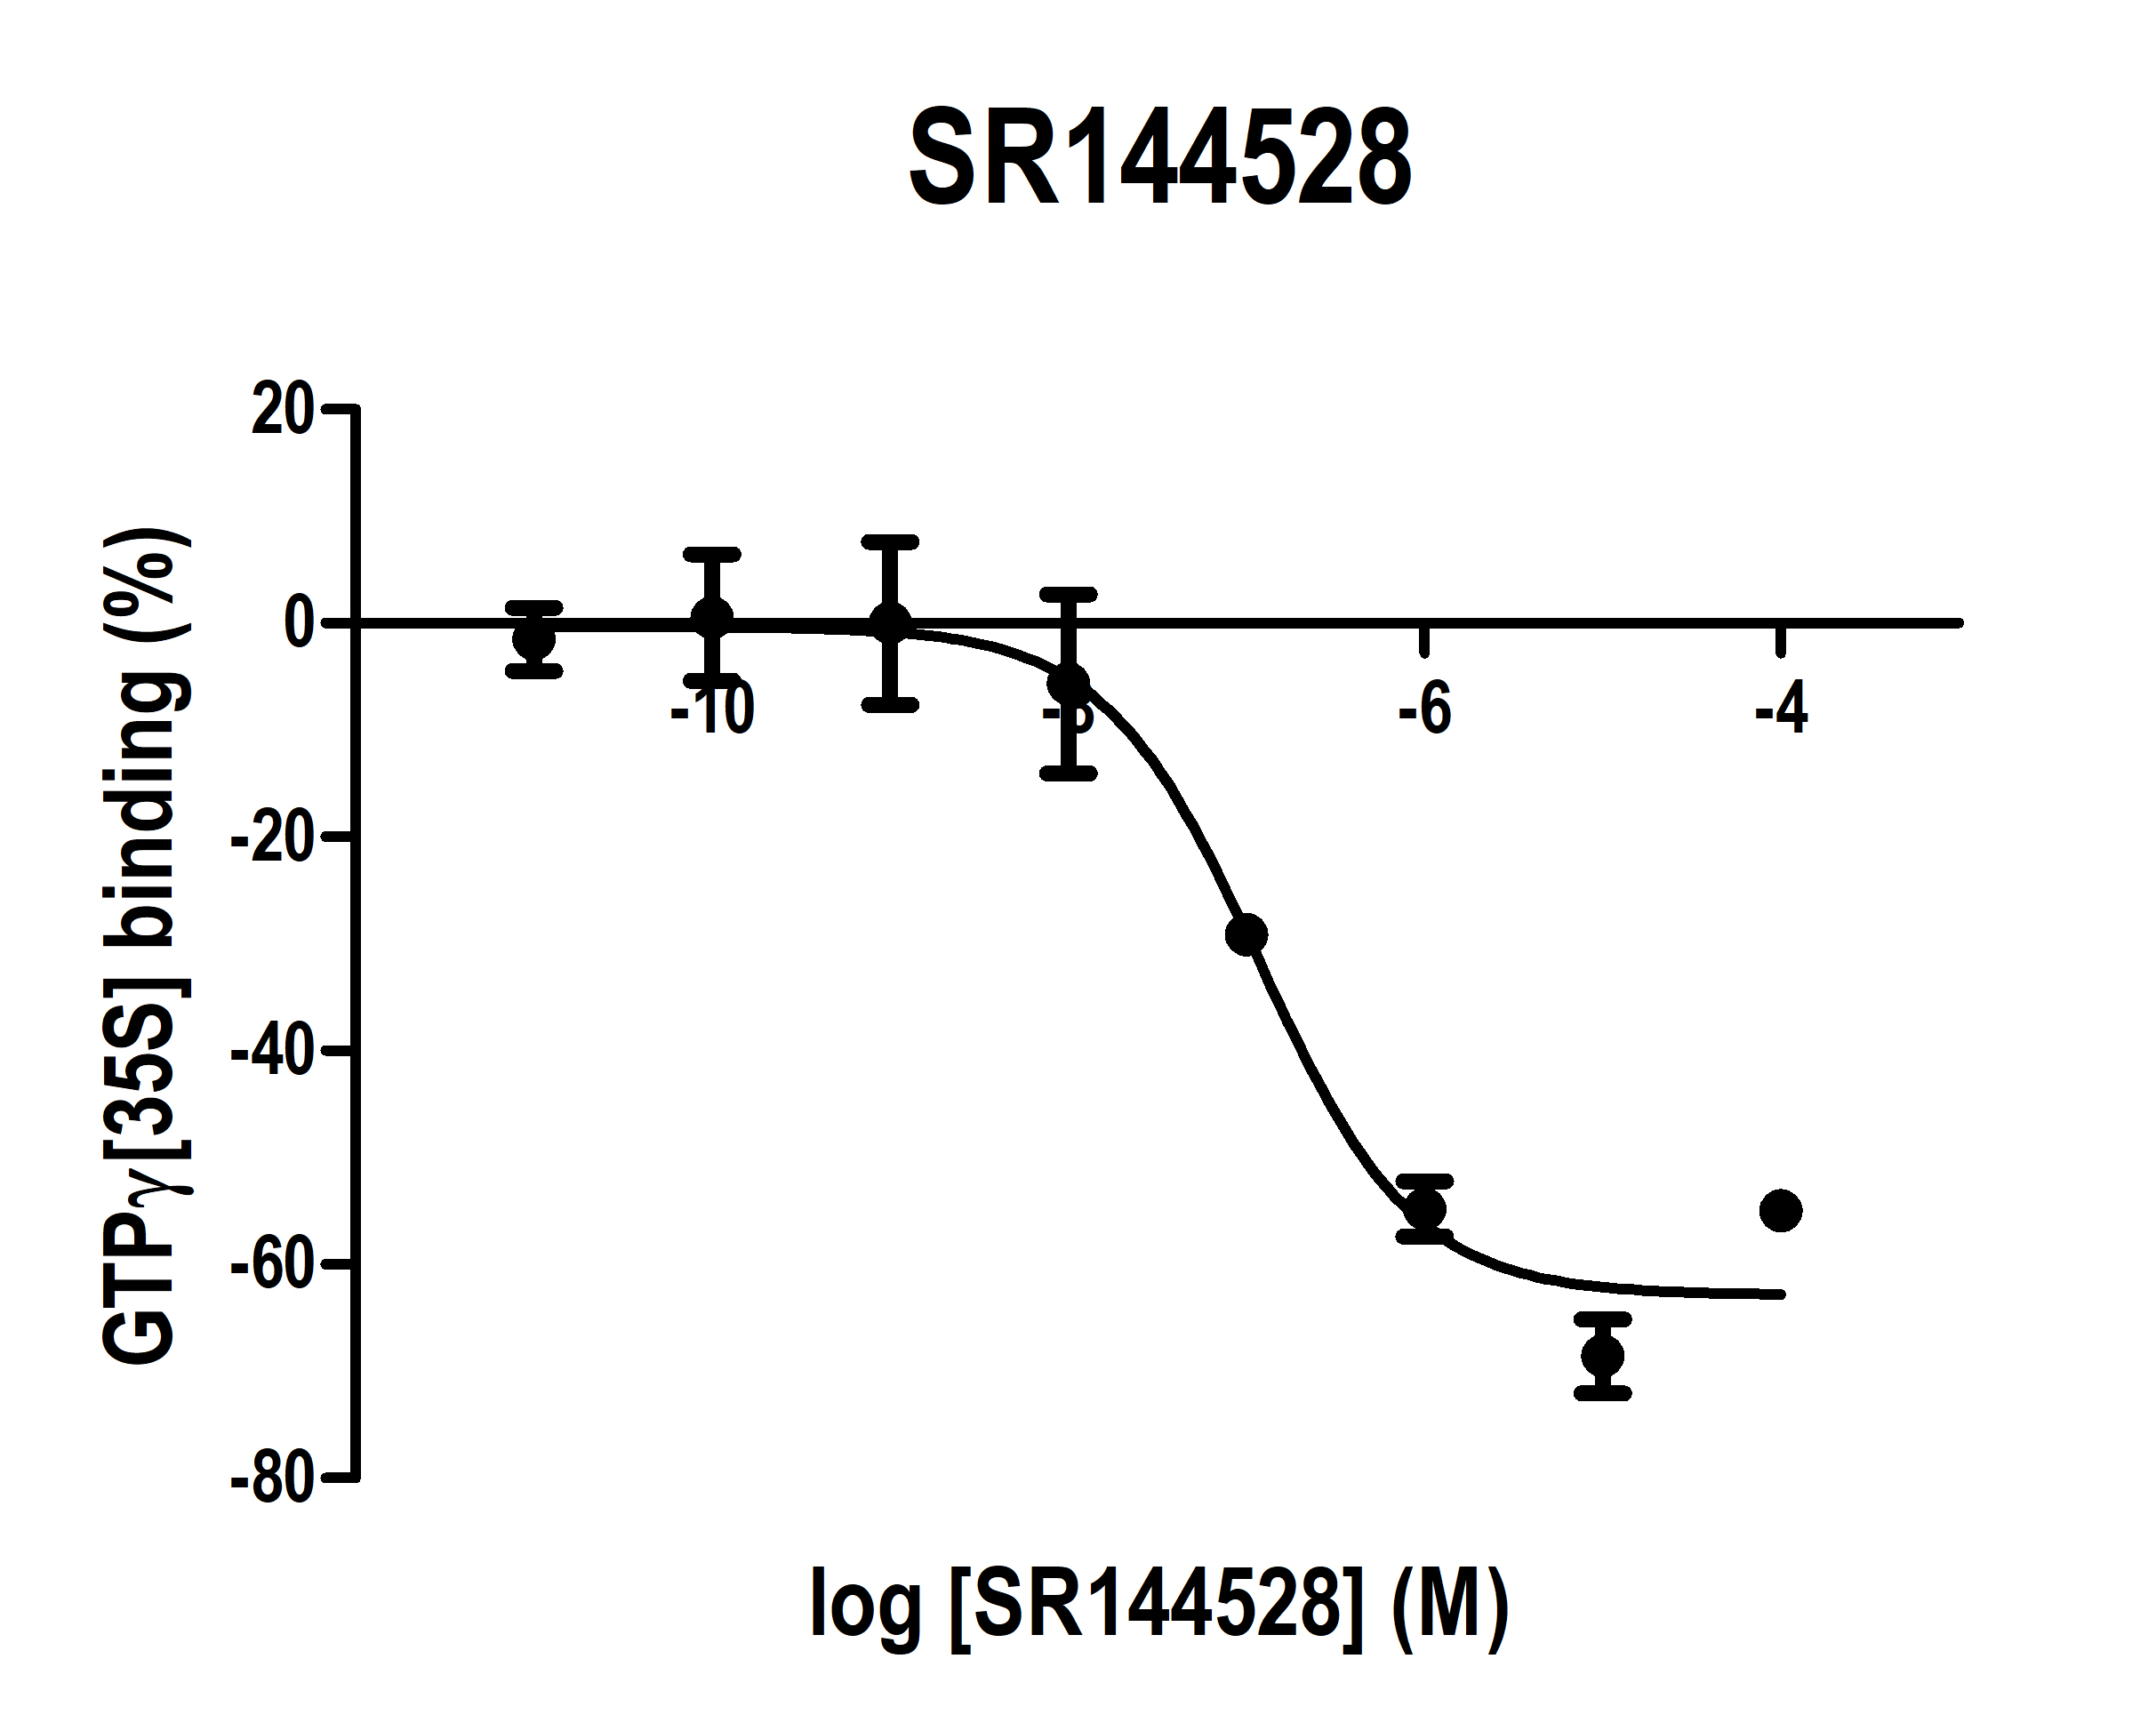
\includegraphics[width=.4\textwidth]{media/1A.jpg}
    }
    \subcaptionbox{\label{fig:1b}}{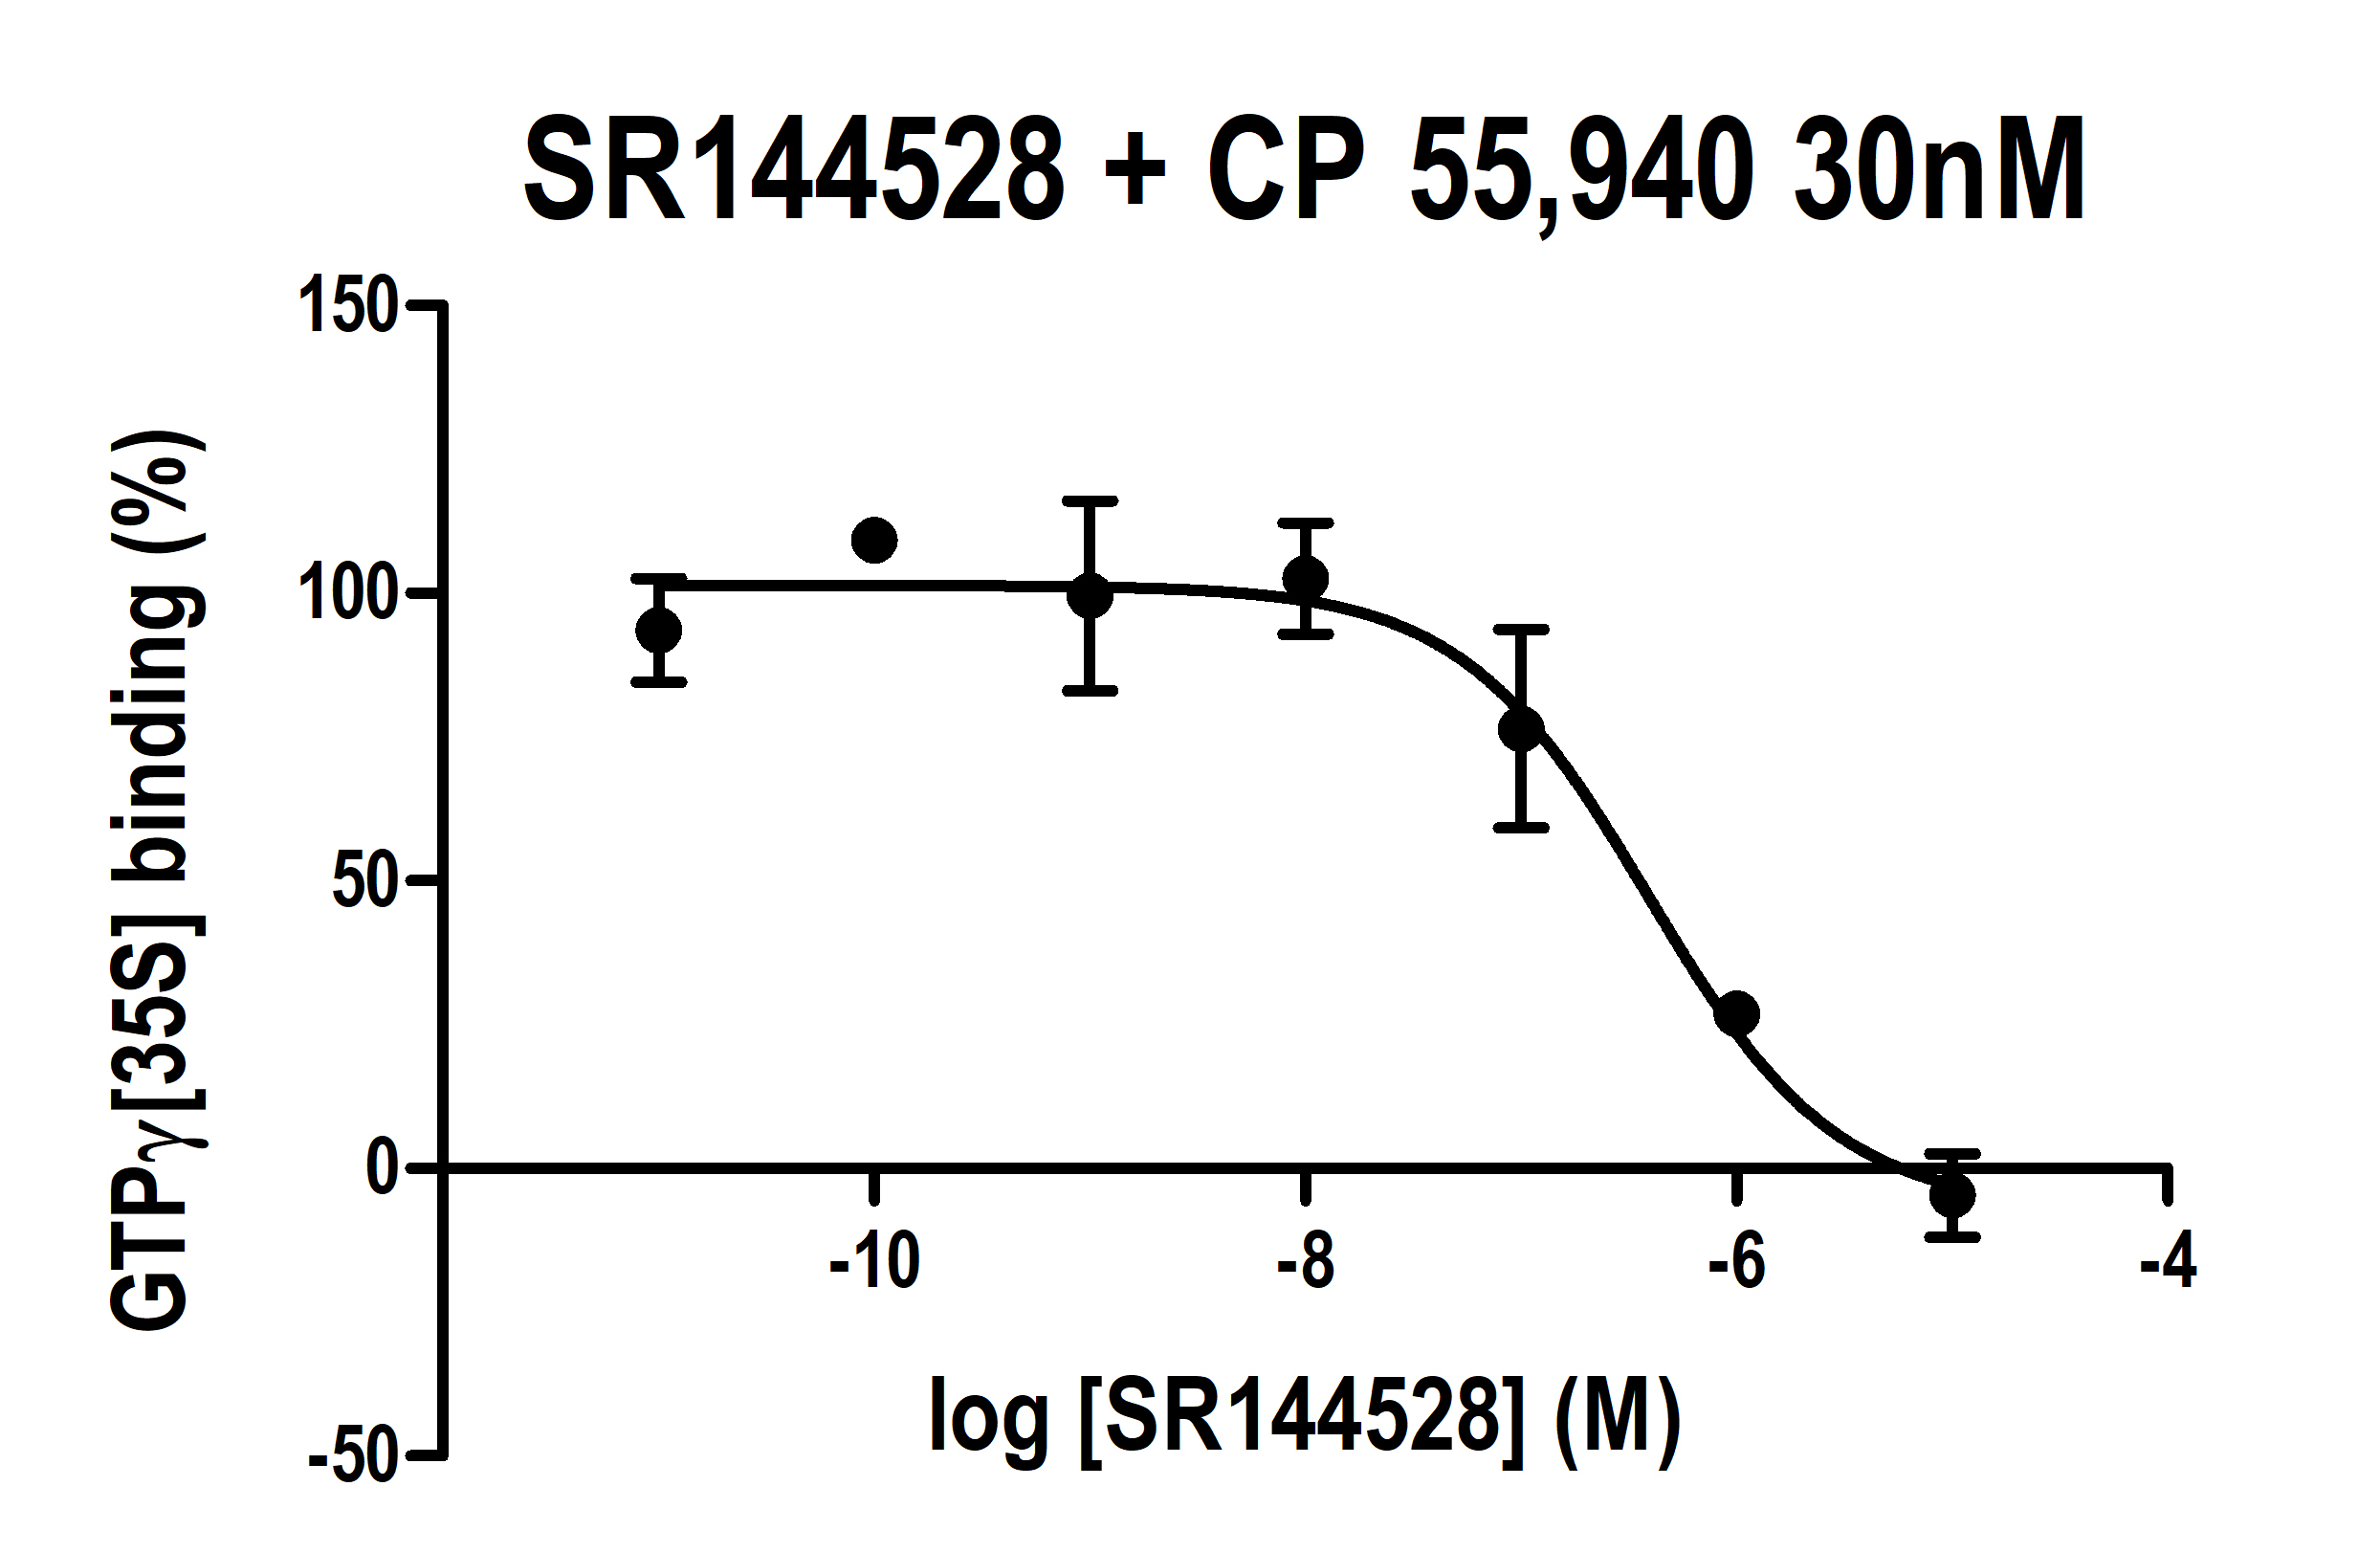
\includegraphics[width=.4\textwidth]{media/1B.jpg}
    }
    \caption{}
    \label{fig:1}
  \end{fullwidth}
\end{figure*}

\begin{figure}[h!]
  \begin{fullwidth}
    \subcaptionbox{\label{fig:2a}}{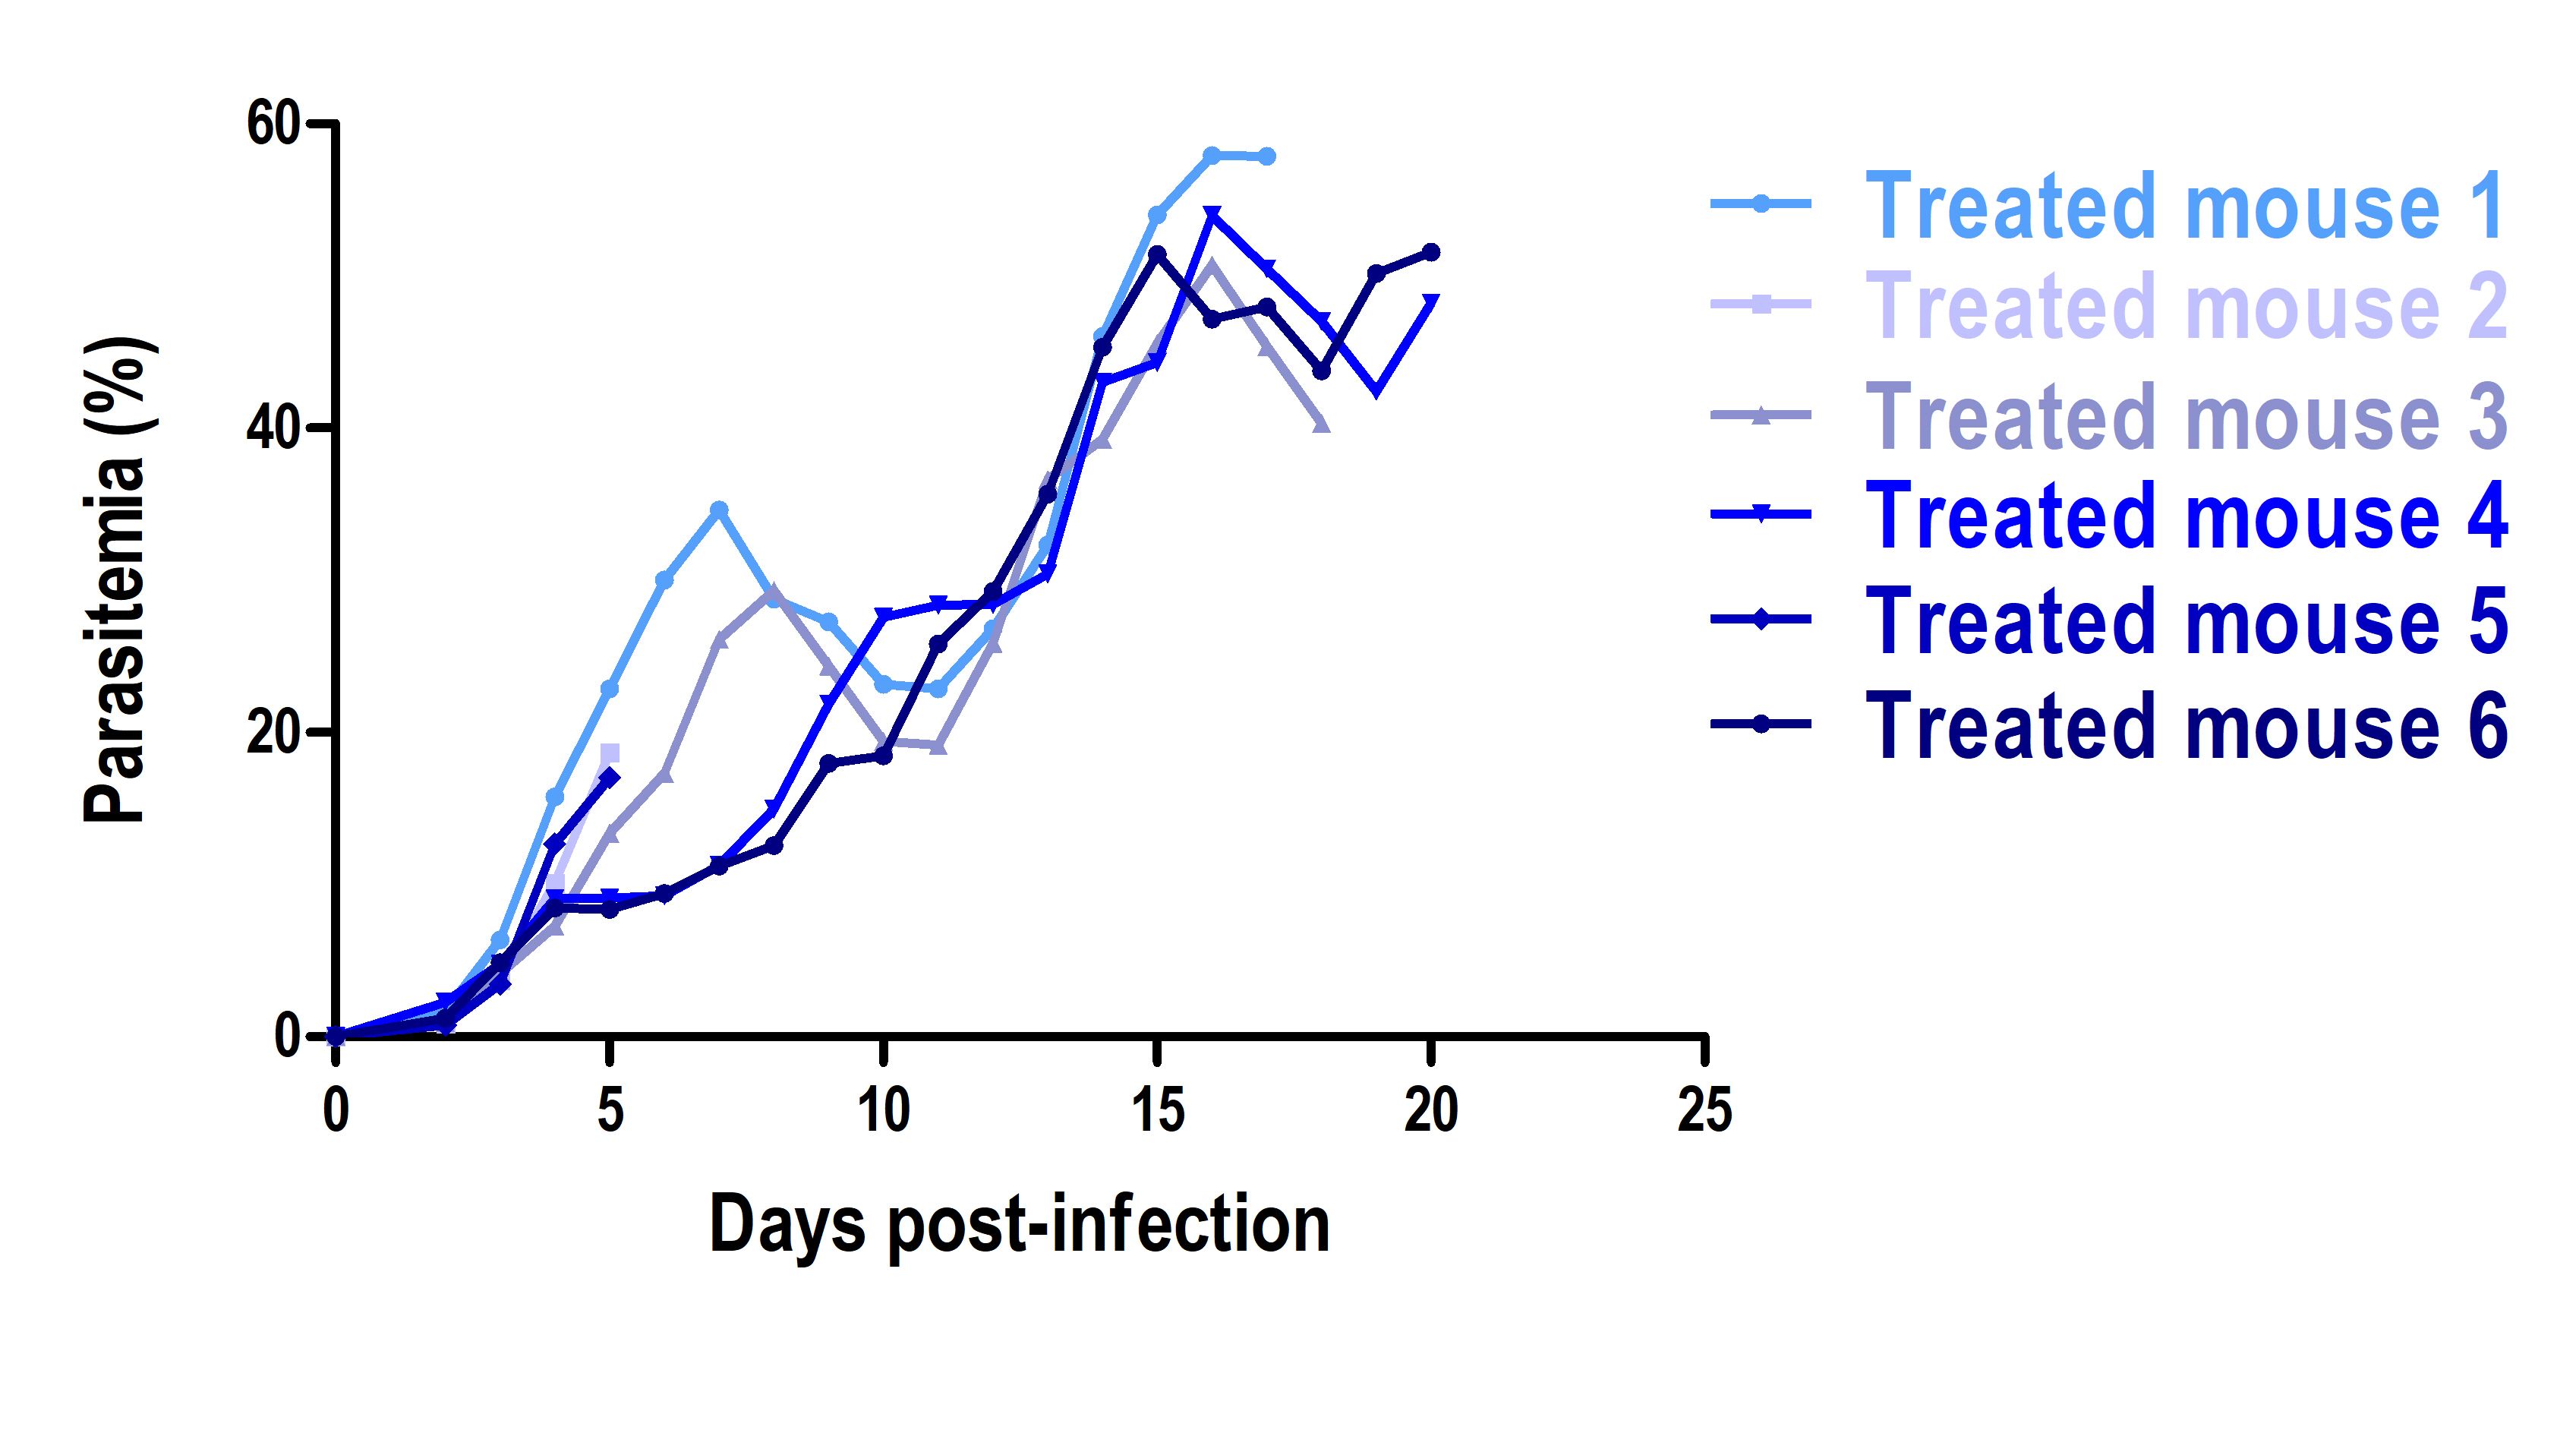
\includegraphics[width=.95\textwidth]{media/2A.jpg}
    }
    \subcaptionbox{\label{fig:2b}}{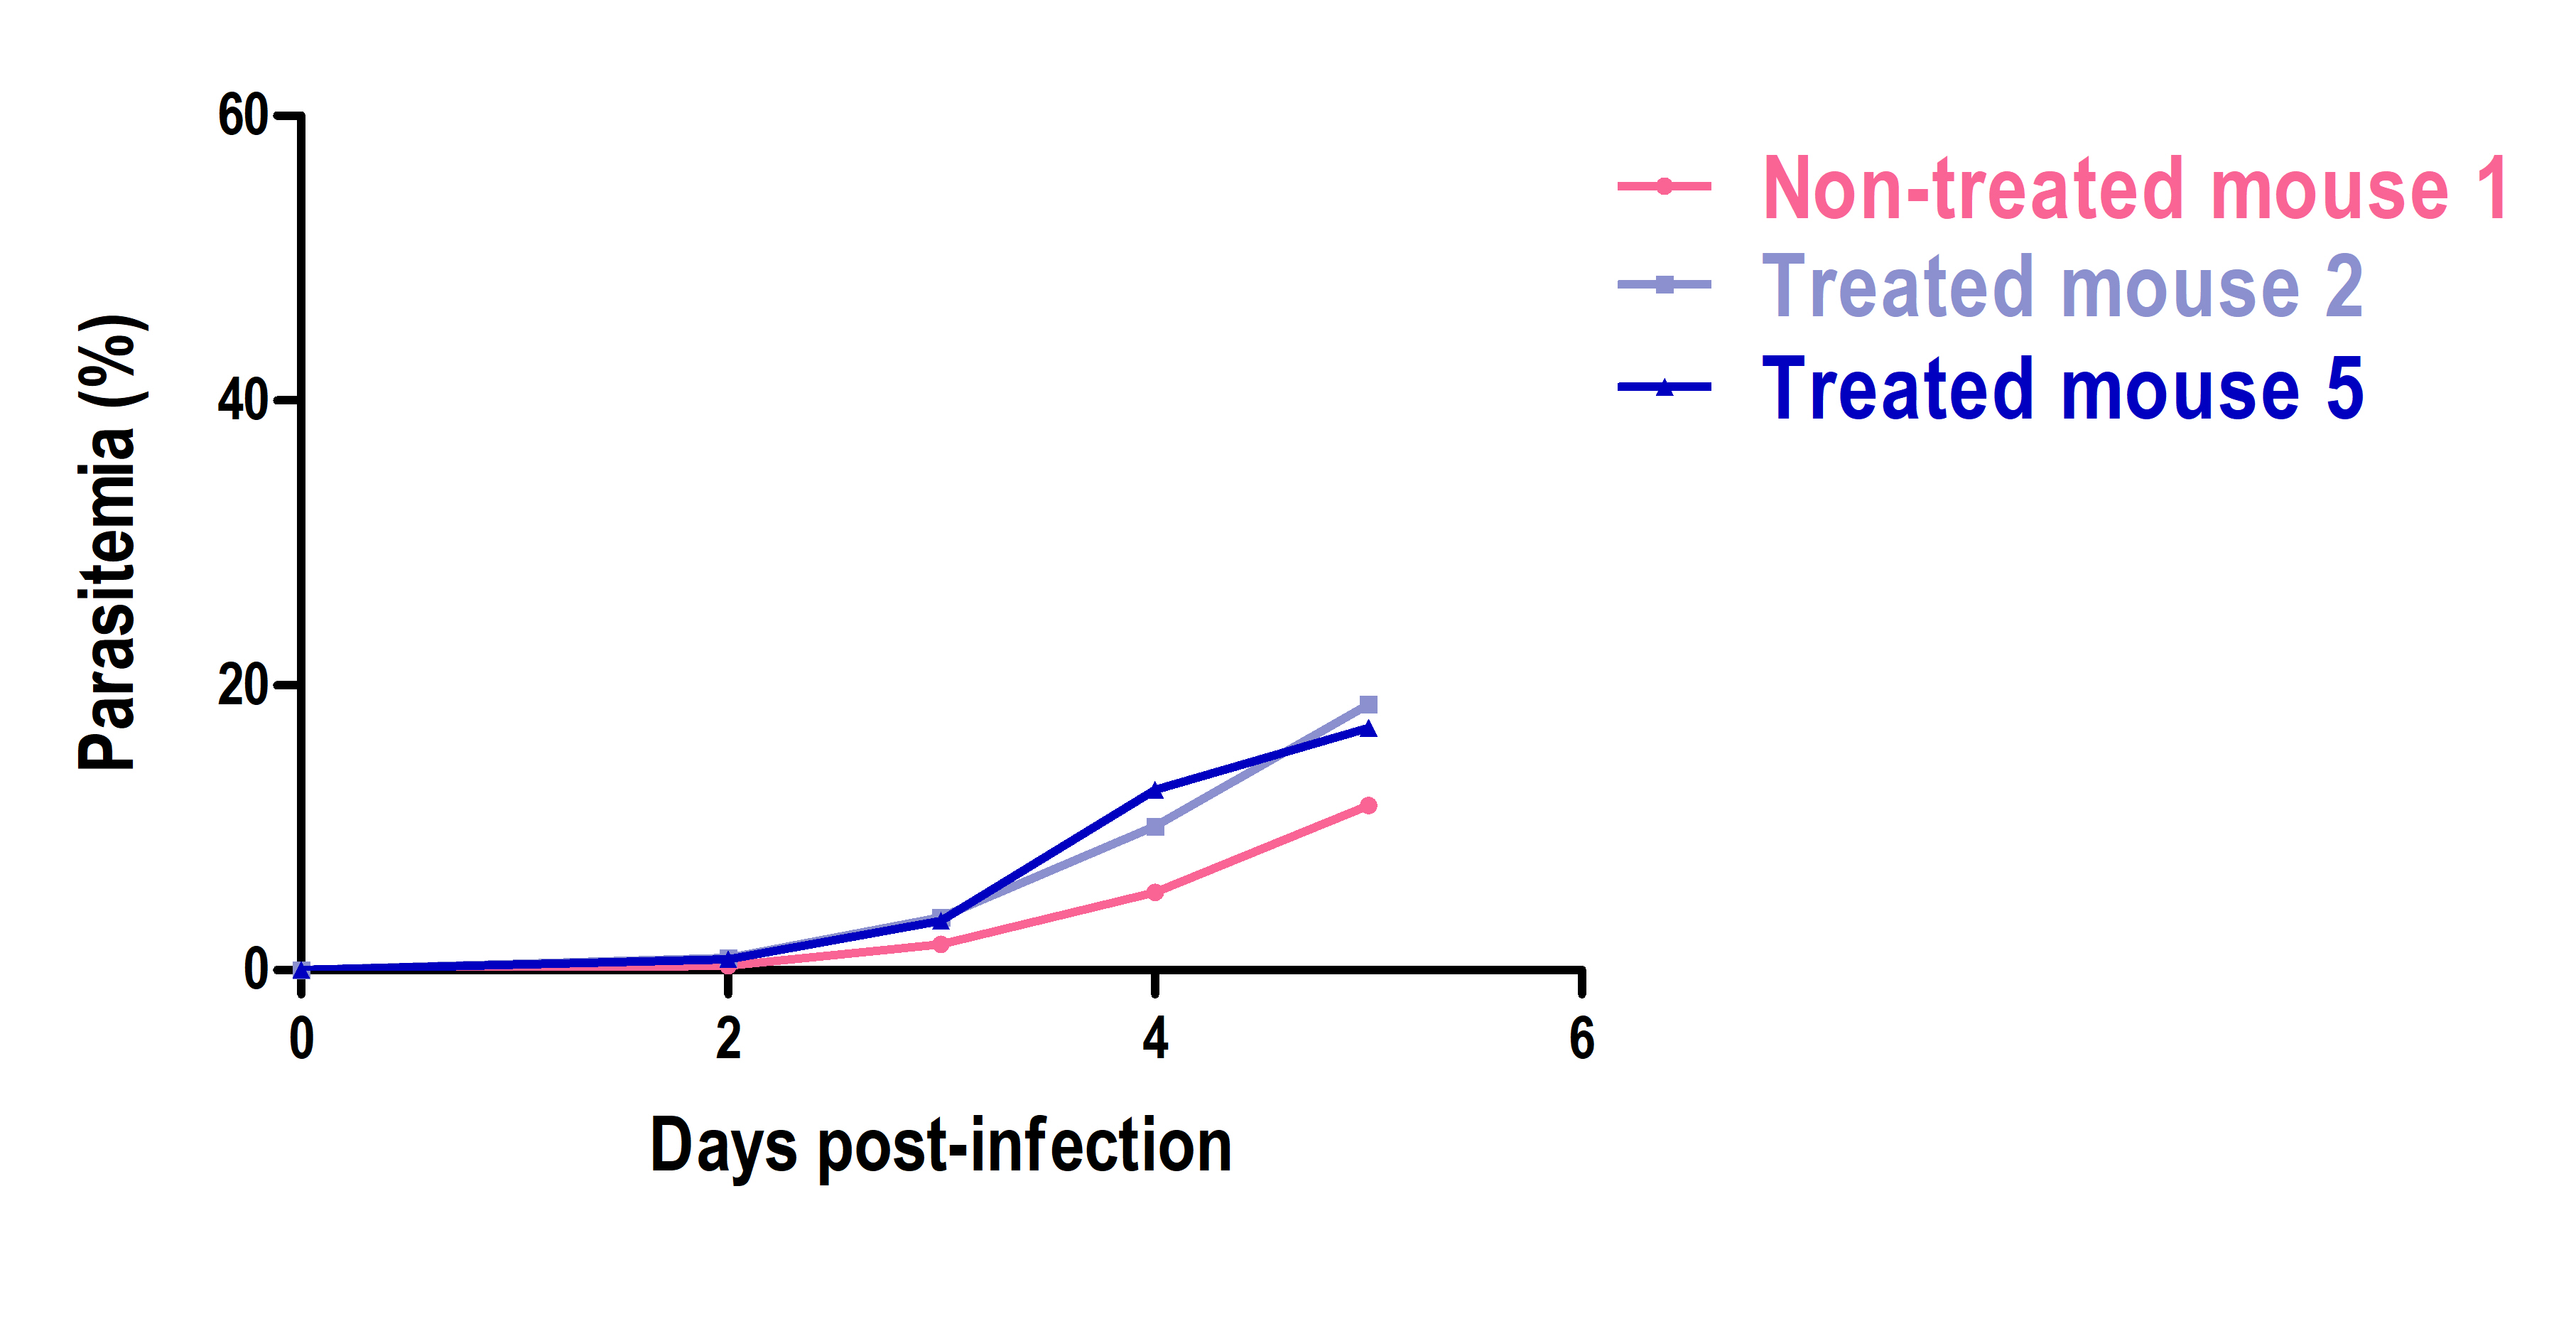
\includegraphics[width=.95\textwidth]{media/2B.jpg}
    }
    \caption{}
    \label{fig:2}
  \end{fullwidth}
\end{figure}



Infection progress was daily monitored daily by staining blood smears with Wright's eosin methylene blue solution (Merck) followed by counting pRBC under the microscope and quantitative determination of percent parasitemia using the PlasmoScore software (version 1.3). Moreover, the neurological performance of the animals was daily evaluated daily in individual mice by recording clinical symptoms including ruffled fur, abnormal gait, tremor, reduced grip strength, affected startle, abnormal visual response, reduced motility, head deviation, hemi- or paraplegia, tendency to roll over on stimulation, back elevation, ataxia, and convulsions. According to previous standardizations of the experimental cerebral malaria \parencite{Martinez2013, Linares2013}, infected animals were grouped in disease stages from I to IV depending on the severity of their neurological signs as follows: STAGE stage I, no neurological symptoms in the first few days of infection; STAGE stage II, incipient symptoms of CM; STAGE stage III, appreciable neurological symptoms; and STAGE stage IV, severe symptoms. After the death of the animals, their brain tissue was immediately removed, fixed in 10\% formaldehyde, and embedded in paraffin. Series of 5 \emph{μm}-thick were cut and stained with hematoxylin and eosin to elucidate and assess histopathological damages.


\section{Results and Discussion}

\begin{originalPurpose}
  Nowadays, the mainstay of the treatment of severe cerebral malaria is the immediate onset of parenteral antimalarial treatment: available drugs include quinolones, antifolates and artemisin-combination therapies. However, despite the effectiveness of antimalarial drugs on treating most malaria related symptoms, their efficacy on promoting survival and preventing neurological damage, mainly in children, is contested. In this scenario, the combination of antimalarial drugs and CNS-acting compounds would be an interesting strategy for the improvement of the neurological outcome in CM patients. Previous studies have shown that the CB2 receptor could be an important modulator of susceptibility in experimental cerebral malaria (ECM). Moreover, therapeutic application of a specific CB2 antagonist also seems to confer increased ECM resistance in wild type mice. Thus, targeting CB2 and blocking its intracellular signaling might be promising for the development of alternative treatment regimens for CM.
\end{originalPurpose}

\subsection{CB\textsubscript{1}/CB\textsubscript{2} receptor binding studies for SR144528}

The CB\textsubscript{1} and CB\textsubscript{2} receptor binding affinities of SR144528 were evaluated by radioligand binding assays carried out by competition with [\textsuperscript{3}H]-CP 55,940 and the data of receptor affinities and selectivity are shown in Table \ref{tab:1}. These data indicate that SR144528 is able tocan bind at the CB\textsubscript{1} receptor with a \emph{Ki} in the high \emph{nM} range, but that it has a higher affinity for the CB\textsubscript{2} receptor, reaching a K\textsubscript{i} value in the low nM range and with a CB\textsubscript{1}/CB\textsubscript{2} ratio of 36.2 (Table \ref{tab:1}).






\subsection{Determination of the functional activity of SR144528 at the CB\textsubscript{2} receptor}

Subsequently, we investigated the efficacy (agonism \emph{versus} antagonism and/or inverse agonism) of SR144528 at the CB\textsubscript{2 }receptor by conducting [\textsuperscript{35}S]-GTPγS binding assays. As expected, SR144528 behaved as inverse agonist of the CB\textsubscript{2} receptor (Fig.~\ref{fig:1a}) with significant values of IC\textsubscript{50} and efficacy (Emax) described in the Table \ref{tab:2}. We also conducted supplementary assays to determine the antagonistic capacity of SR144528 in the presence of the CB\textsubscript{1}/CB\textsubscript{2} agonist CP55,940 (30 \emph{nM}), which revealed a strong capability for this compound to antagonize the effects of CB\textsubscript{2} agonists (Fig.~\ref{fig:1b}).


\subsection{In vivo assessment of SR144528 therapeutic potential in ECM}




The preclinical assessment of the therapeutic effect of SR144528 as a CB\textsubscript{2} receptor antagonist was carried out in the \emph{P. berghei }ANKA ECM murine model. Several studies have widely highlighted the phenotypic similarities between the experimental CM model of \emph{P. }\emph{berghei}\emph{ }ANKA infecting C57BL/6 mouse and the neurological disease progression in humans \parencite{DeSouza2010, Hunt2003, Lou2001,Medana2006}. To follow disease and infection progress in this model, peripheral blood parasitemia, and neurological phenotype alterations were monitored on a daily monitored basis in treated and non-treated mice.

Peripheral blood parasitemia values are shown in Figure 2 for both, non-treated (Fig.~\ref{fig:2a}) and SR144528 treated mice (Fig.~\ref{fig:2b}). Values are individually plotted to show potential outliers responses, if any. Comparing non-treated and treated animals, a certain level of individual heterogeneity was observed in both groups. Thus, some animals showed a marked blood hyperparasitemia from day 10 post-infection, whereas others died early on died in the first 5 days after infection with low parasitemia levels (around 15\%).

\begin{figure}[h!]
  \begin{fullwidth}
    \raggedright
    \subcaptionbox{\label{fig:3a}}{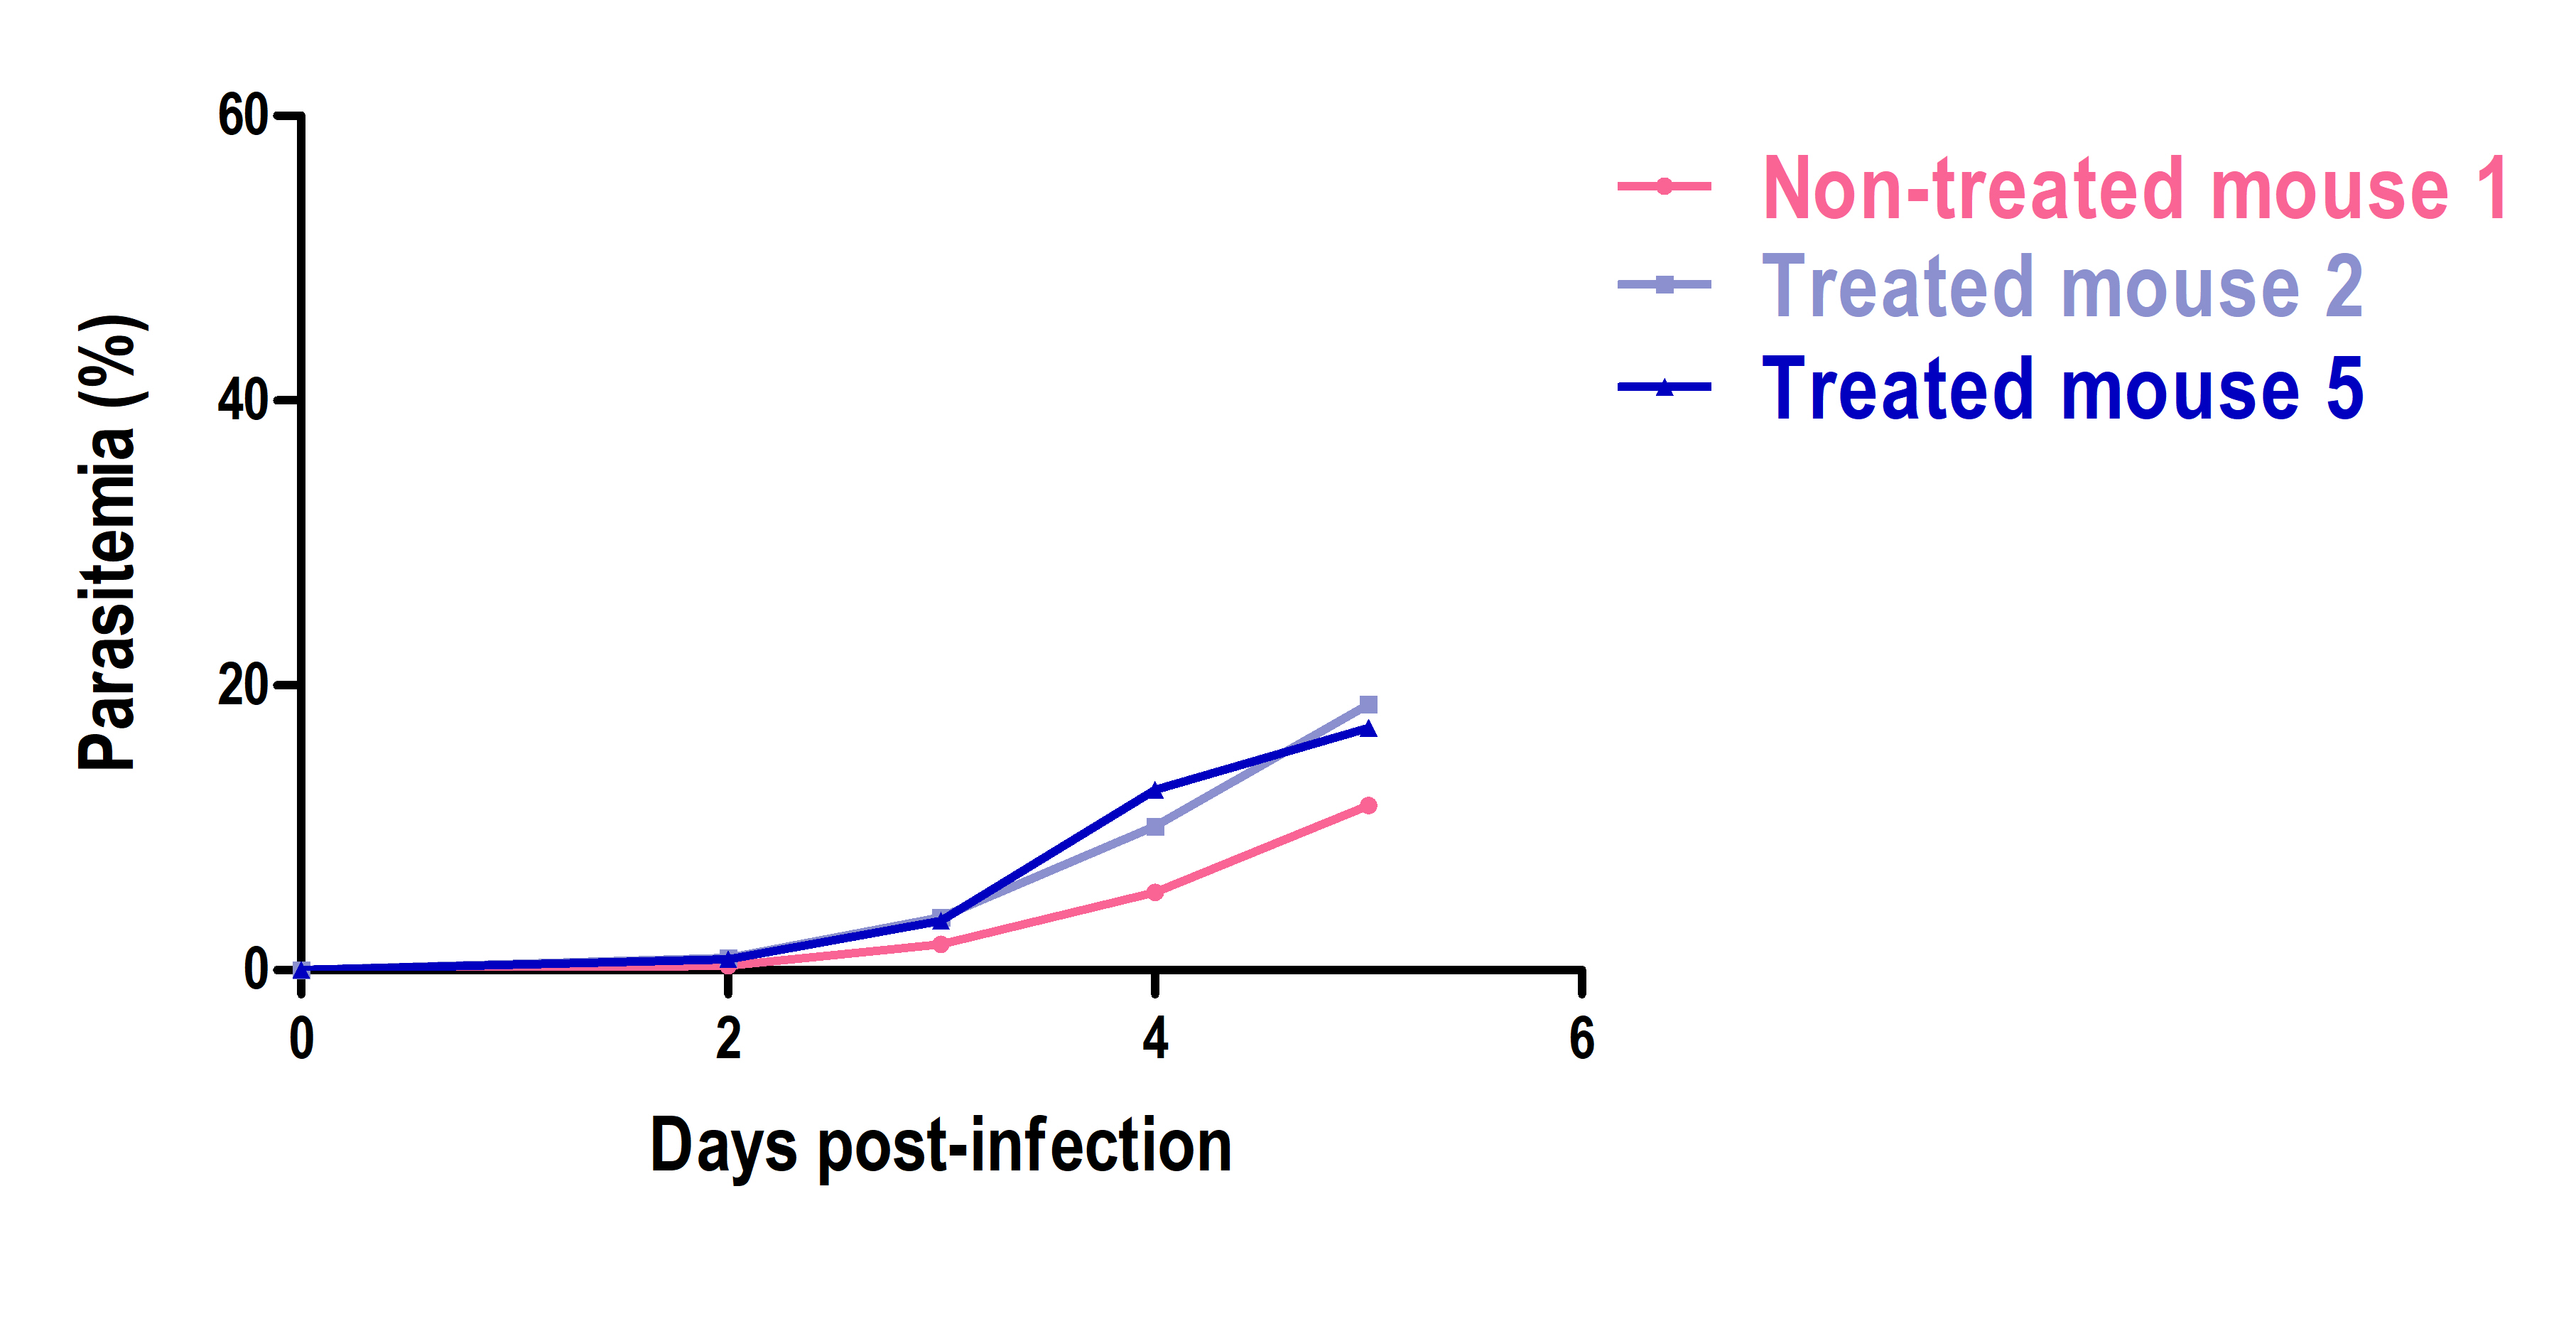
\includegraphics[width=.95\textwidth]{media/3A.jpg}
    }
    \subcaptionbox{\label{fig:3b}}{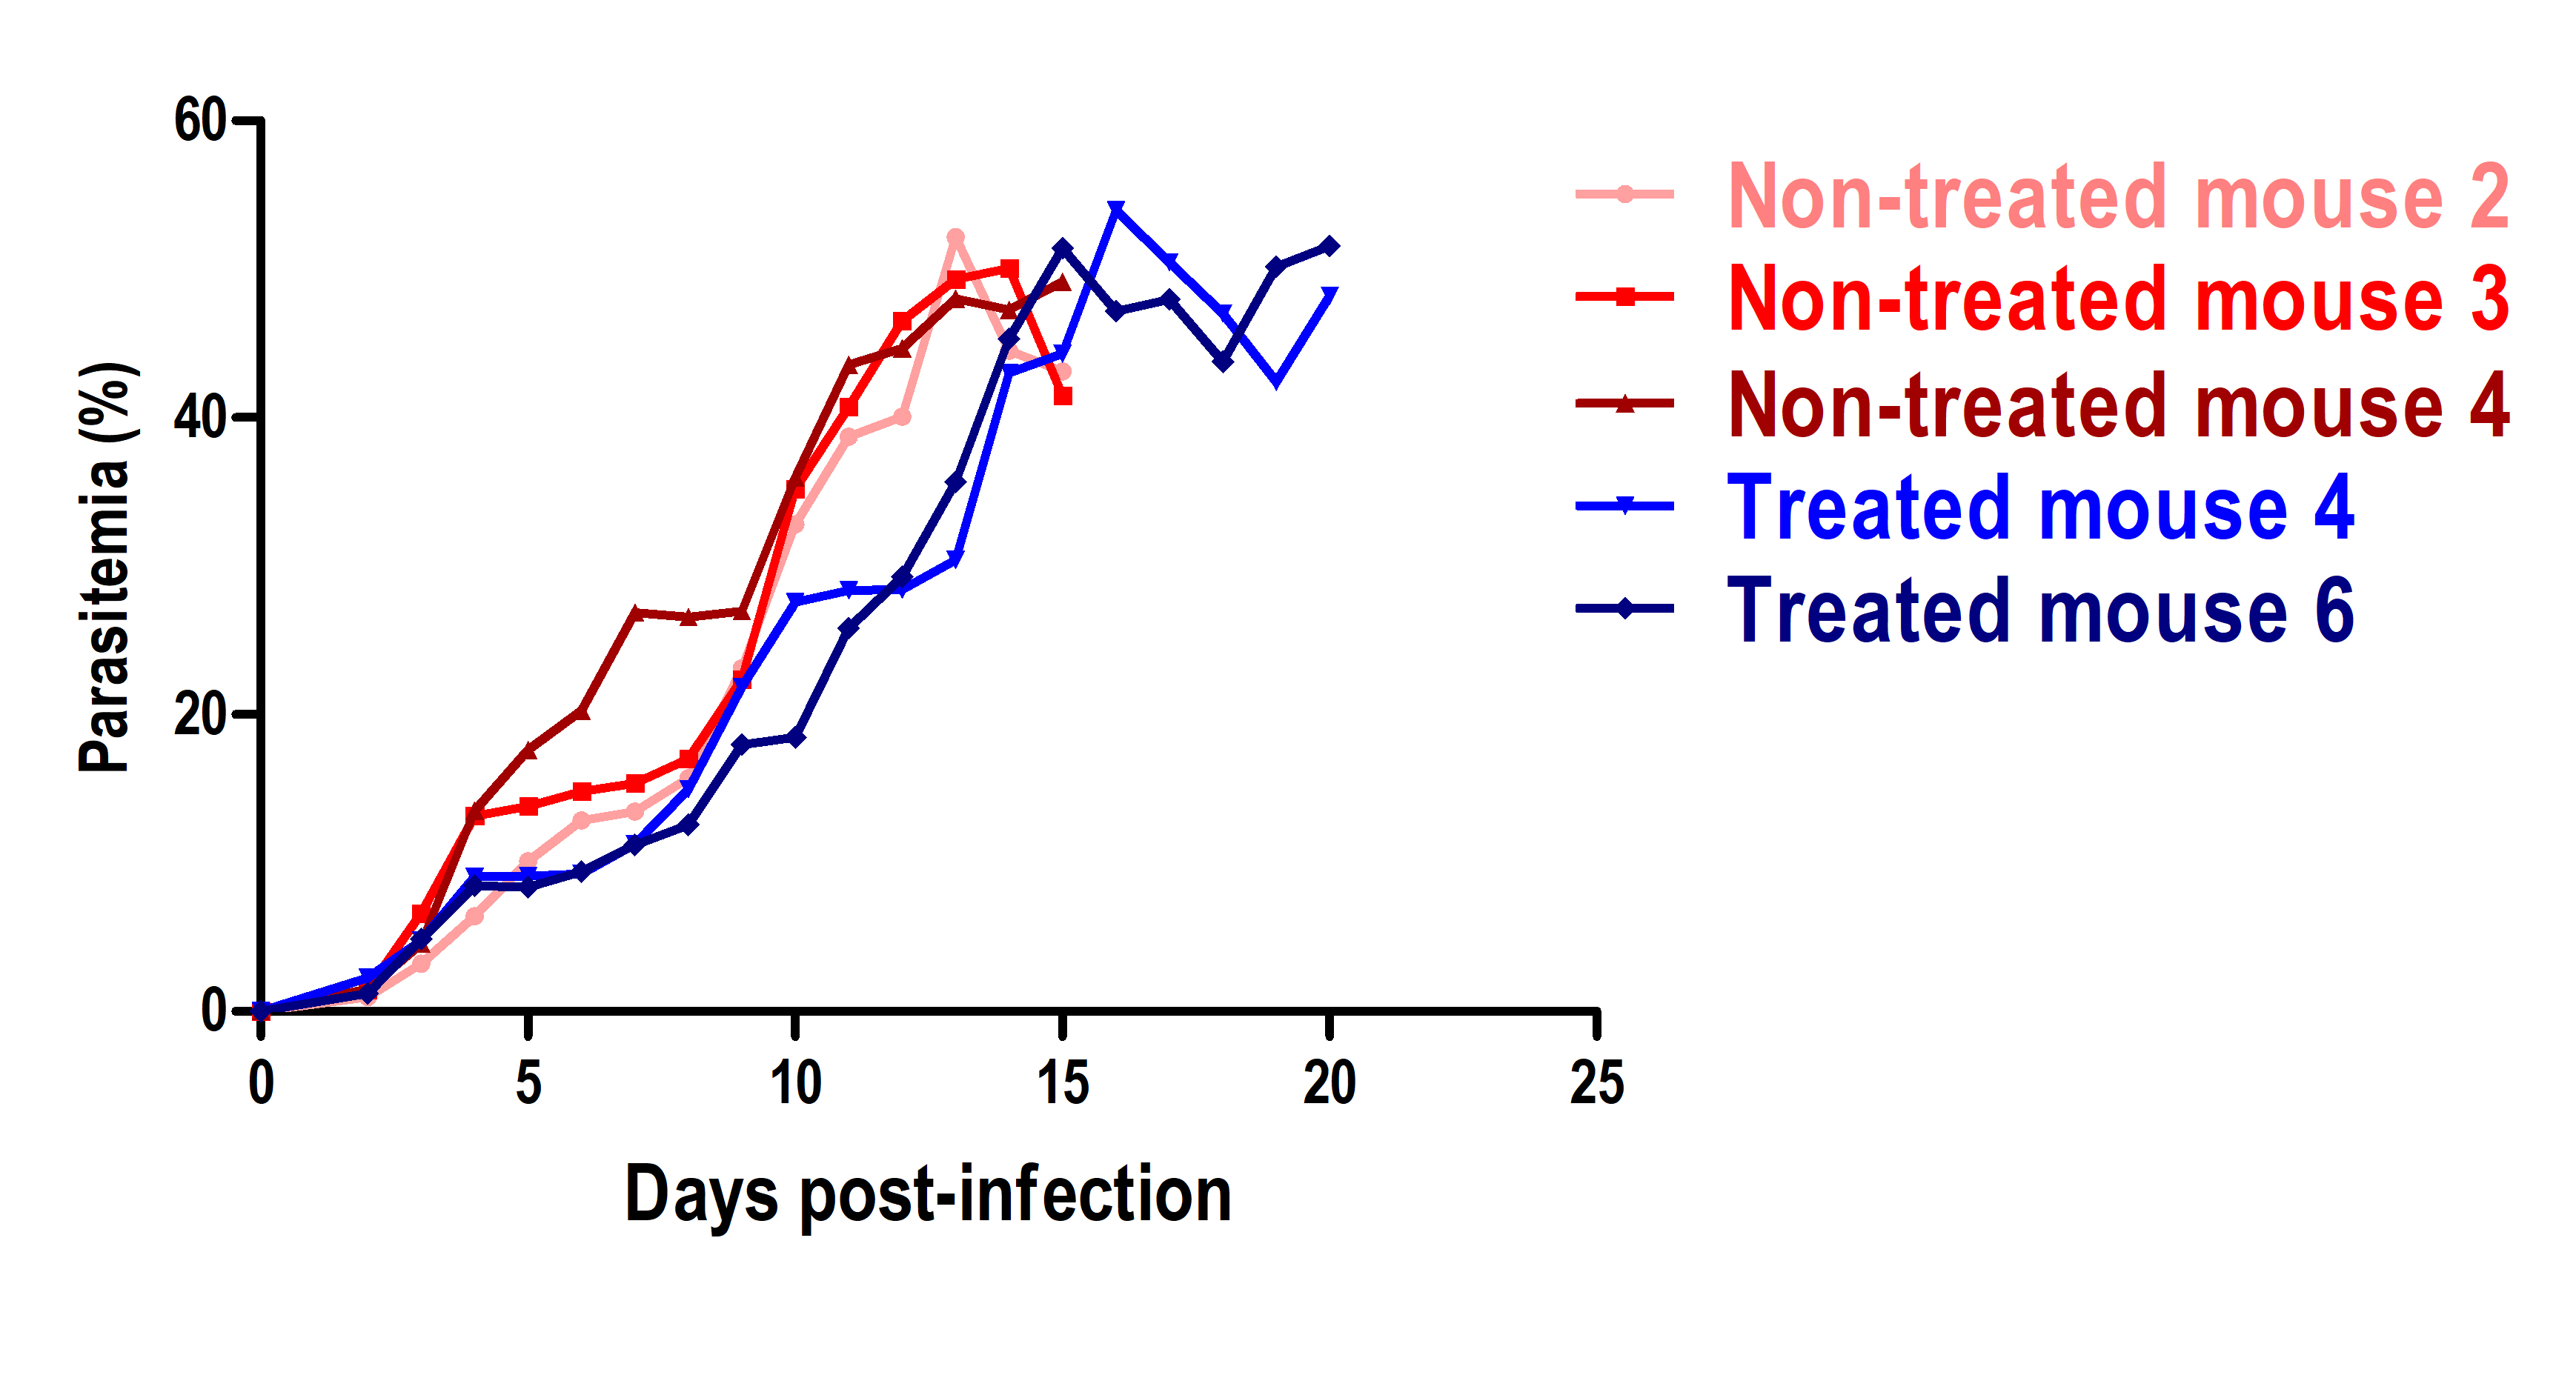
\includegraphics[width=.95\textwidth]{media/3B.jpg}
    }
    \subcaptionbox{\label{fig:3c}}{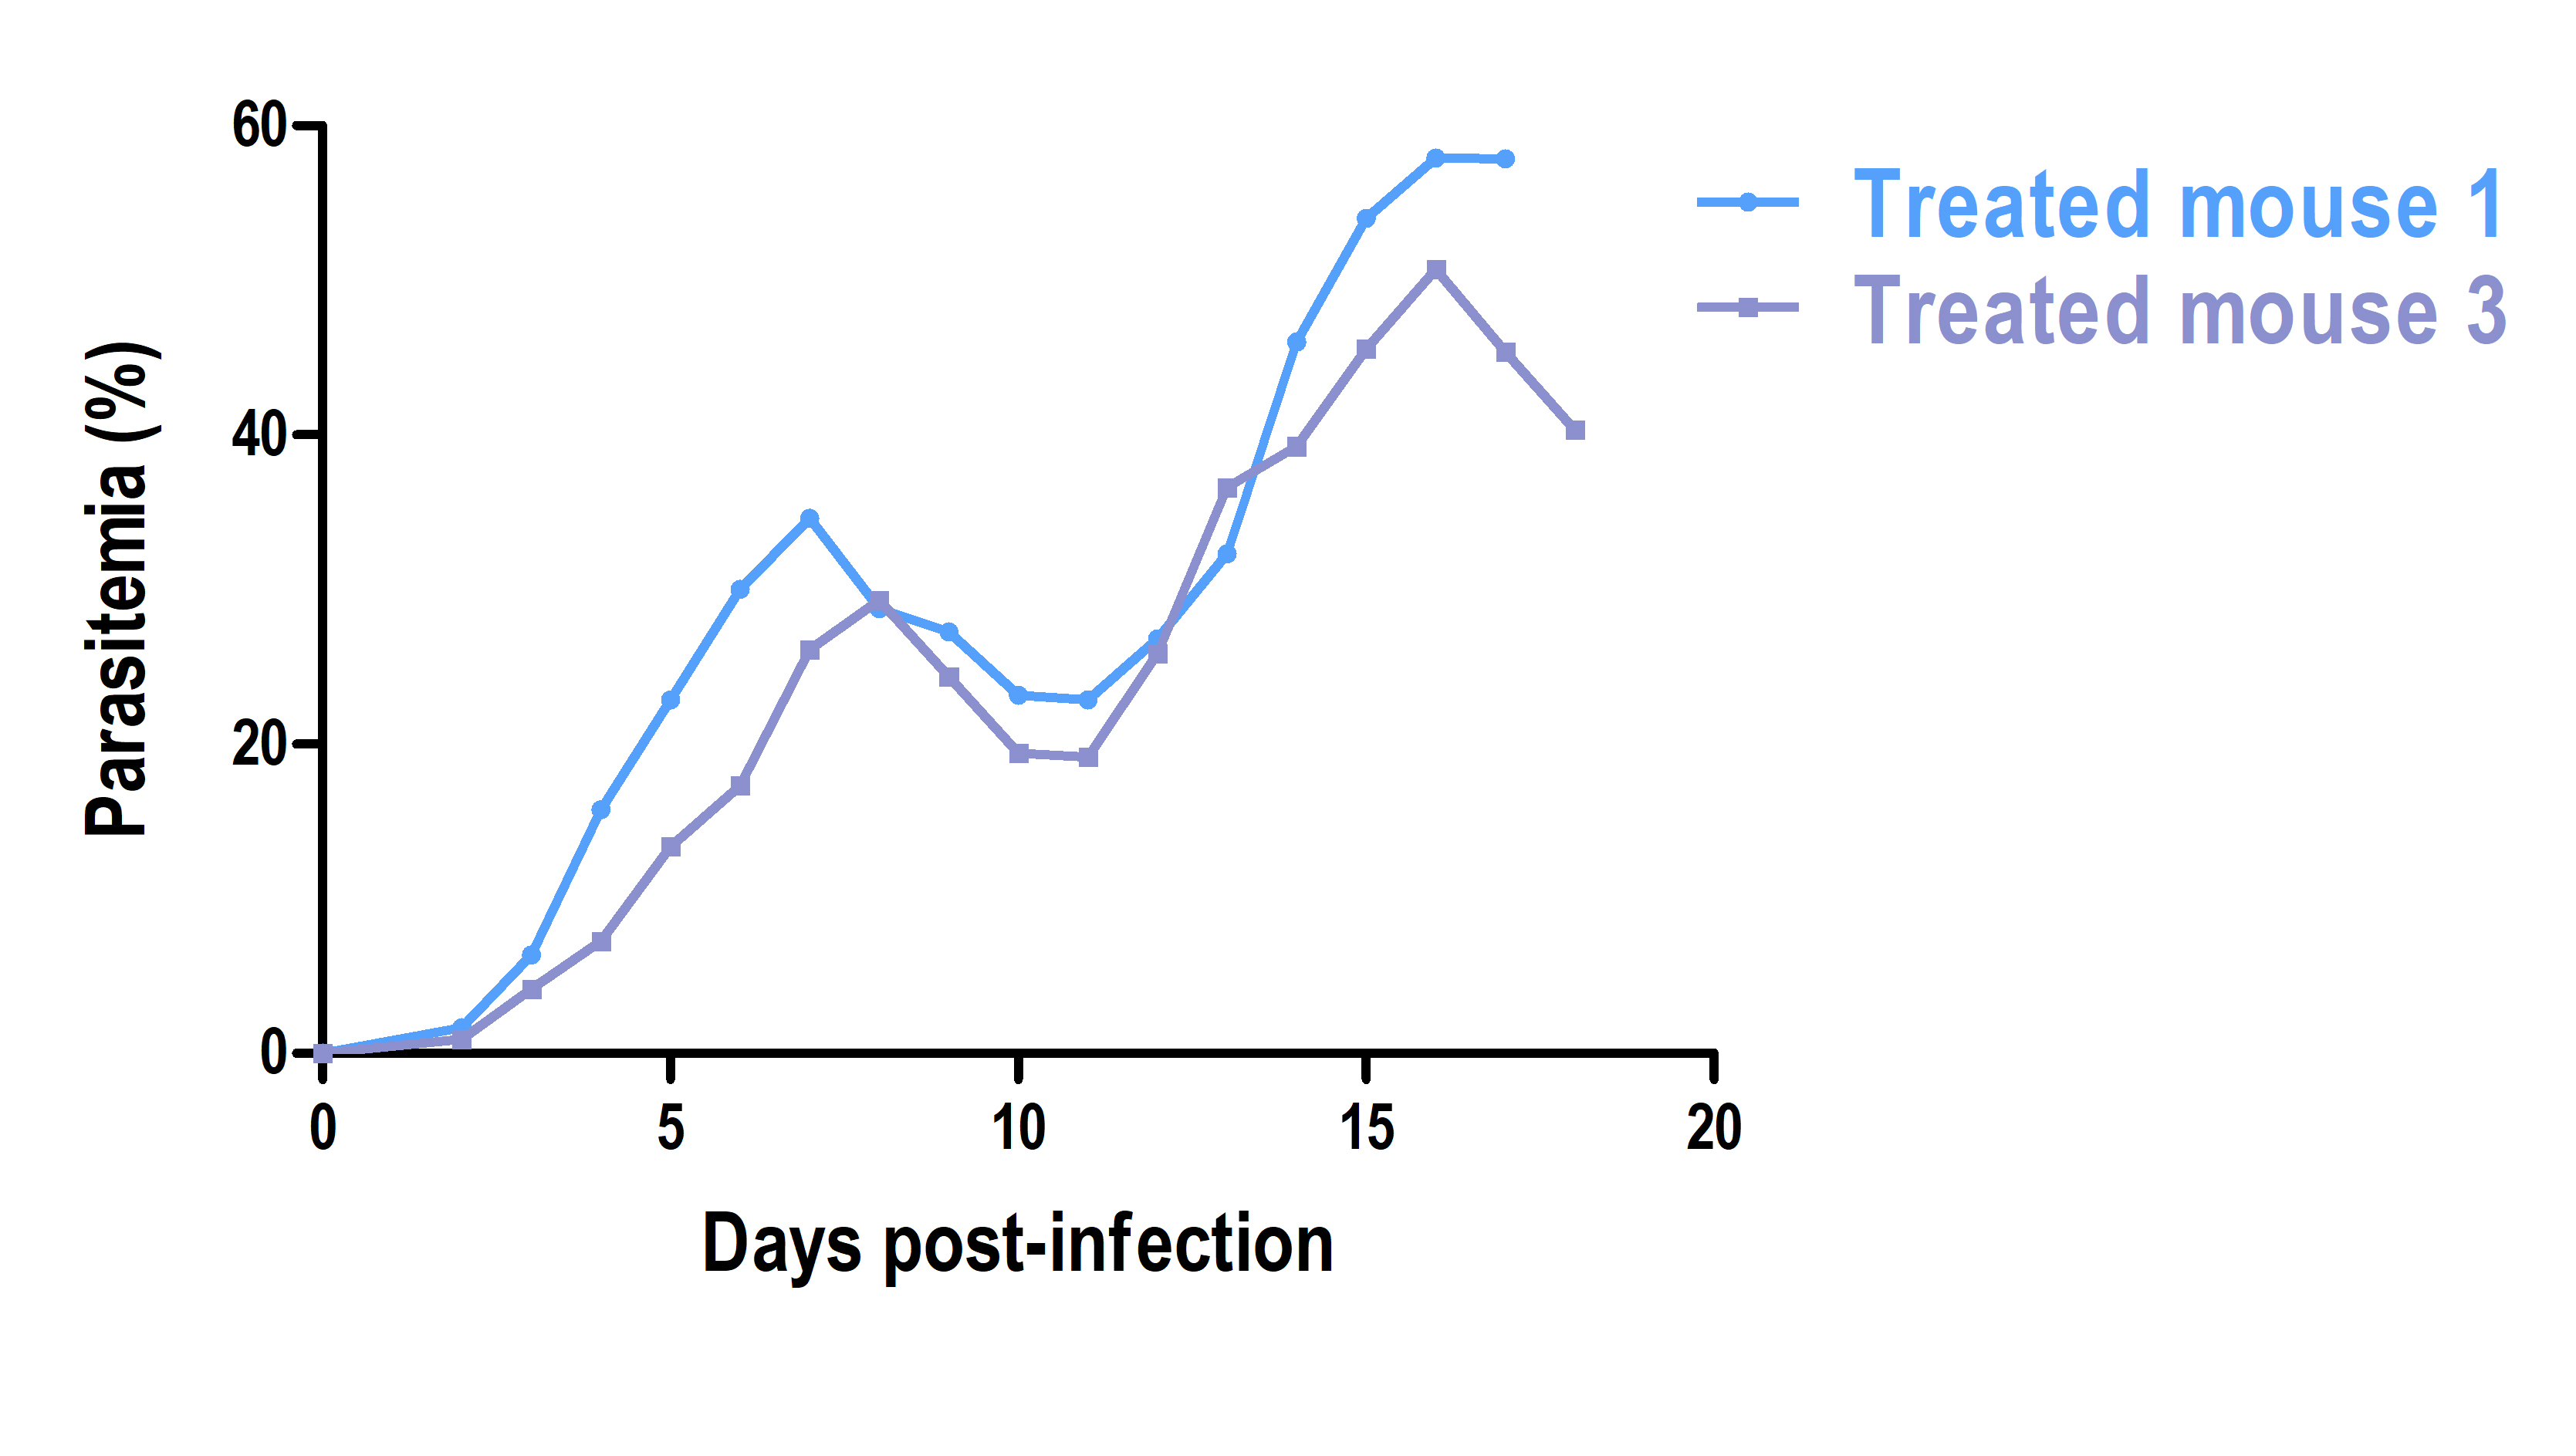
\includegraphics[width=.95\textwidth]{media/3C.jpg}
    }
    \caption{}
    \label{fig:3}
  \end{fullwidth}
\end{figure}
Behavioral characterization of neurological alterations underlying CM progression, allowed to the conclusionconclude that,, based on the non-treated mice results, the \emph{P. berghei} ANKA-C57BL/6 model can lead to the acquisition of either non-cerebral malaria (NCM) with high levels of peripheral blood parasitemia or CM. Thus, considering the parasitemia curves and the corresponding phenotypes, we classified disease progress into three different clinical groups: a first group of CM, a second of NCM, and a third designated as `mixed group'. Consequently, we separately reanalyzed the data according to these three clinical groups (Fig.~\ref{fig:3}).

The \textbf{experimental group of CM }(Fig.~\ref{fig:3a}) included the non-treated mouse 1 and the treated mice 2 and 5. These three animals , considering phenotypic alterations, blood parasitemia levels and disease progression, were classified as CM cases, considering their phenotypic alterations, blood parasitemia levels, and disease progression. These mice showed phenotypic features of brain pathology, that can be assigned to a disease stage II on day 5 post-infection, with incipient neurological alterations such as ruffled fur, head deviation, tremor, and increased respiratory rate. These mice died on day 6 post-infection with low parasitemia levels around 11-18\%.


The \textbf{NCM group} (Fig.~\ref{fig:3b}) included the non-treated mice 2, 3, and 4 and the treated mice 4 and 6. These animals were classified as NCM cases, based on parasitemia development and disease progression, showing no signs or behaviors of neurological disorder were classified as NCM cases. All individuals in this group evolved similarly and died within the same time interval between days 15 and 21 post-infection due to a strong hyperparasitemia around 49-53\% that caused a strong weight loss and weakness of the animals.




The \textbf{`mixed group' }(Fig.~\ref{fig:3c}) enclosed treated mice 1 and 3. In these two 2 mice, the progression of the disease took place in three different phases, clearly associated with their parasitemia level profiles: a first stage of CM between days 1-7 post-infection; a second phase of recovery between days 8 and 11; and a third stage in which the animals acquired NCM, from day 12 post-infection until death. In phase I, the animals developed a phenotypic and behavioral evolution similar to the CM group. On day 7 post-infection, concurring with a parasitemia peak around 25-30\% (Fig.~\ref{fig:3c}) showed clinical manifestations of stage III CM, including ruffled fur, back elevation, head deviation, ataxia, slight hemi-paralysis of the hindlimbs, and lack of response to stimuli. Nevertheless, these two animals did not progress to coma and death but from day 8 post-infection, the animals entered on what can be considered a phase II with a tendency to recovery by the observed decrease in parasitemia levels to 19-22\%. This reduction in parasitemia values was also reflected in the neurological signs with recovered mobility, response to stimuli and no tremor or head deviation. Finally, from day 12 post-infection, their clinical and parasitemia evolution matched with the mice included in the NCM group, acquiring very high levels of parasitemia, around 50-55\%, without neurological alterations but dying at day 17-19 post-infection due to critical weakness, marked weight loss and severe anemia.


According to this clustering, SR144528 administration to the CM and NCM groups had no therapeutic effect. The evolution of the infection did not change between treated and non-treated mice in CM and NCM groups, finally ending in death at the same time, either by CM or by severe anemia, respectively (Figs.~\ref{fig:3a}-\ref{fig:3b}). However, in the `mixed group', it can be observed that the treatment might have a slight and transient favorable effect, reducing temporarily parasitemia with remission of neurological signs associated with CM (Fig.~\ref{fig:3c}).


\begin{figure}[t]
  \begin{fullwidth}
    \raggedright
    \subcaptionbox{\label{fig:4a}}{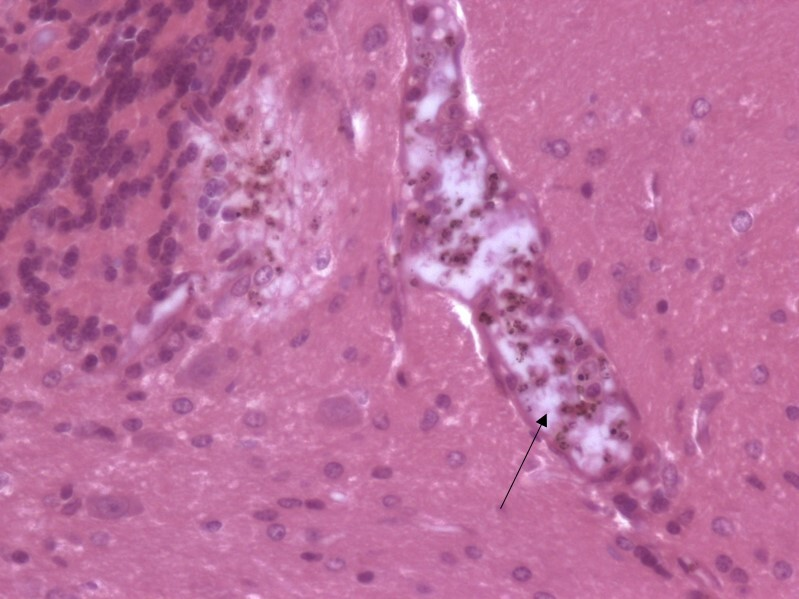
\includegraphics[height=0.36\linewidth]{media/4A.jpg}
    }
    \subcaptionbox{\label{fig:4b}}{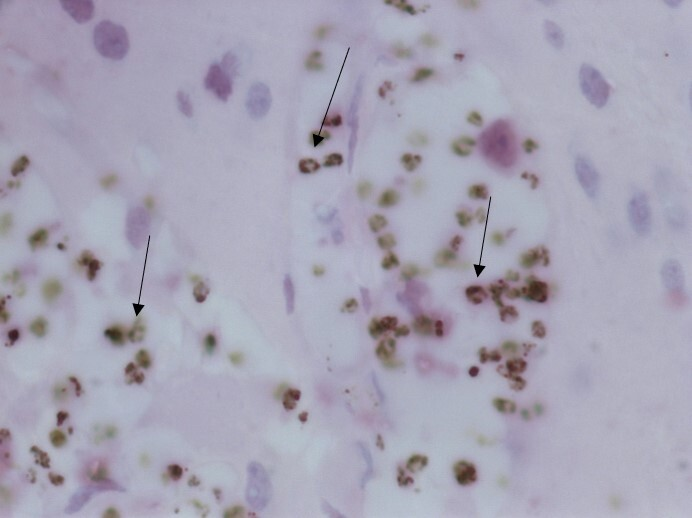
\includegraphics[height=0.36\linewidth]{media/4B.jpg}
    }
    \subcaptionbox{\label{fig:4c}}{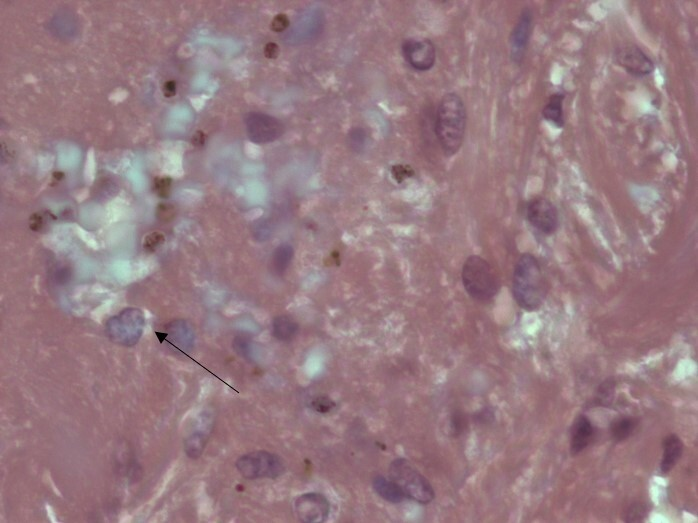
\includegraphics[height=0.36\linewidth]{media/4C.jpg}
    }
    \subcaptionbox{\label{fig:4d}}{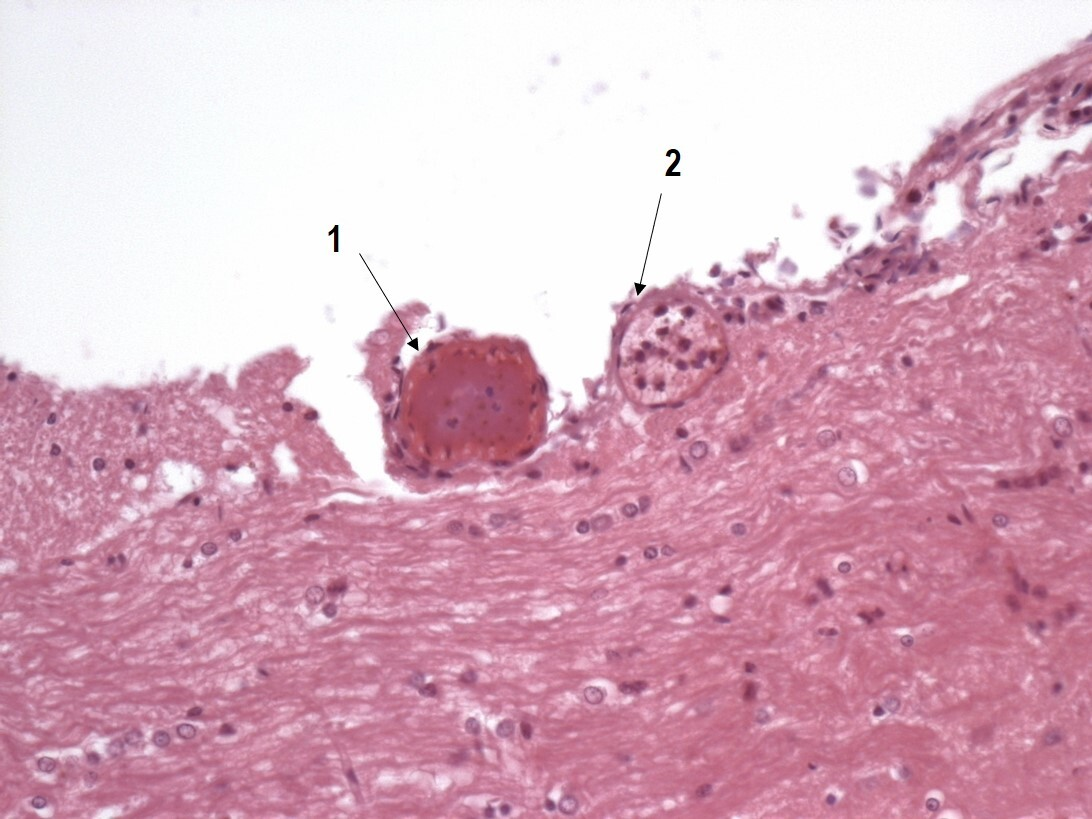
\includegraphics[height=0.36\linewidth]{media/4D.jpg}
    }
    \subcaptionbox{\label{fig:4e}}{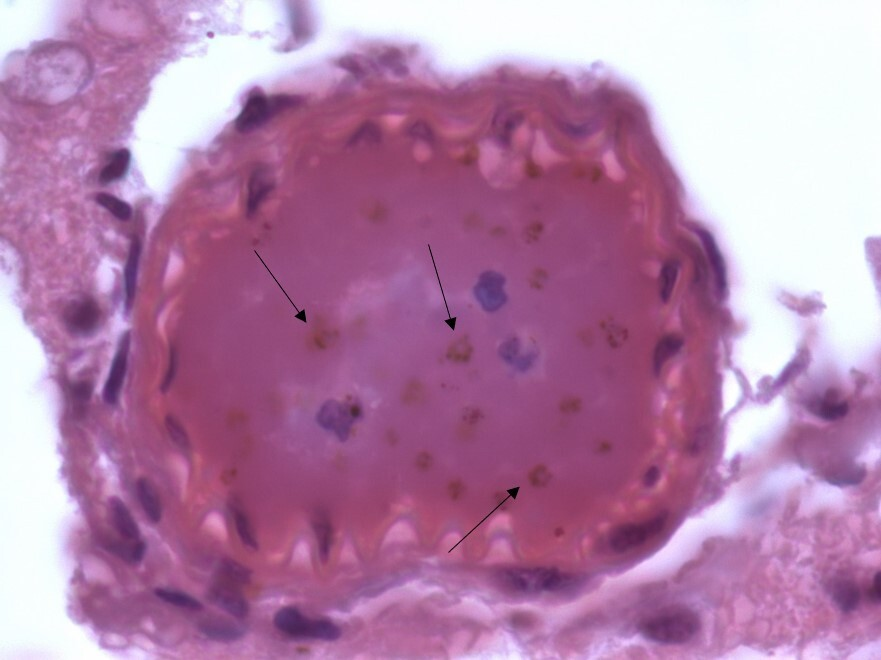
\includegraphics[height=0.36\linewidth]{media/4E.jpg}
    }
    \subcaptionbox{\label{fig:4f}}{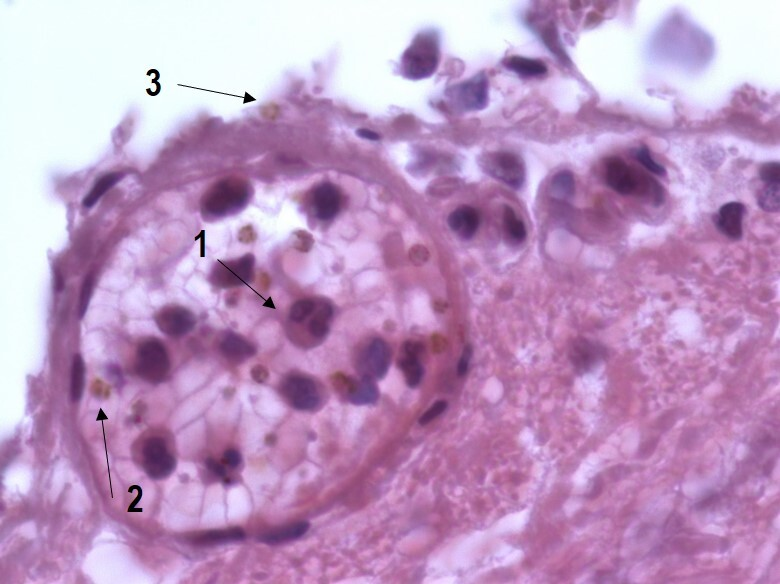
\includegraphics[height=0.36\linewidth]{media/4F.jpg}
    }
    \caption{}
    \label{fig:4}
  \end{fullwidth}
\end{figure}

Furthermore, post-mortem studies showed histopathological features that agreed the classification into 3 three groups based on the clinical manifestations above established. Mice included in the CM group showed clear signs of cerebral alterations at meningeal, cerebellar, and cortical level (Fig.~\ref{fig:4}). Remarkable clusters of inflammatory cells can be observed in several blood vessels at the white and gray matter and meninges, as well as sequestration of pRBC with mature forms of the parasite in the cerebral vasculature (Figs.~\ref{fig:4a}-\ref{fig:4b}). Interestingly, typical erythrocyte Rosseting (Fig.~\ref{fig:4c}), i.e., aggregations of noninfected erythrocytes and pRBCs contributing to the microvascular obstruction, support further signs of severe malaria \parencite{Ross2007} in this CM group. Besides, there were signs of blood brain barrier (BBB) disruption with leukocyte and parasitic extravasation to the brain tissue, diffuse microhemorrhages and areas of edema and thrombosis (Figs.~\ref{fig:4d}-\ref{fig:4f}). No distinctive histopathological differences were observed between the brain sections of the treated and non-treated animals included in the CM group.

Mice classified within the NCM group, either SR144528 treated or non-treated, have minimal brain damage with diffuse microhemorrhages but without meningeal involvement (Fig.~\ref{fig:5a}). No parasite sequestration or clusters of circulating inflammatory cells were identified (Fig.~\ref{fig:5b}). There were was neither no evidence of disruption of the BBB. As in the previous group, no differences were observed in brain sections between non-treated animals (non-treated mice 2, 3, and 4) and treated ones (treated mice 4 and 6) that undergone NCM form upon \emph{P. berghei} infection.

\begin{figure}[t!]
  \begin{fullwidth}
    \centering

    \subcaptionbox{\label{fig:5a}}{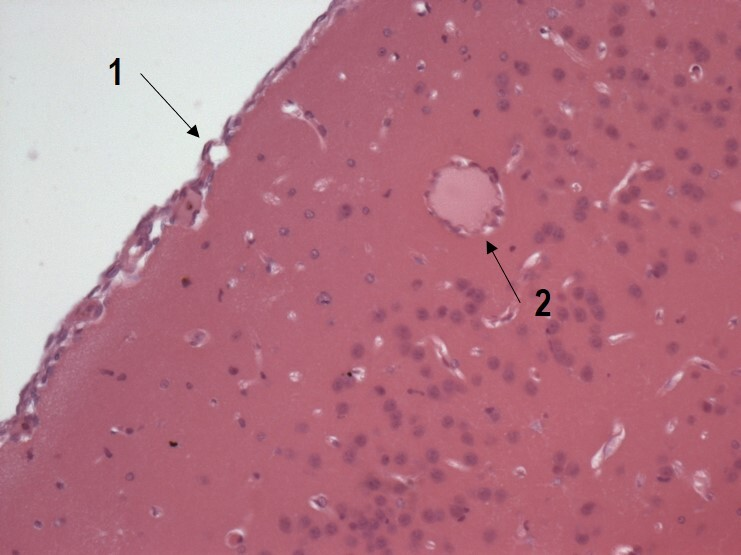
\includegraphics[width=.9\linewidth]{media/5A.jpg}
    }
    \subcaptionbox{\label{fig:5b}}{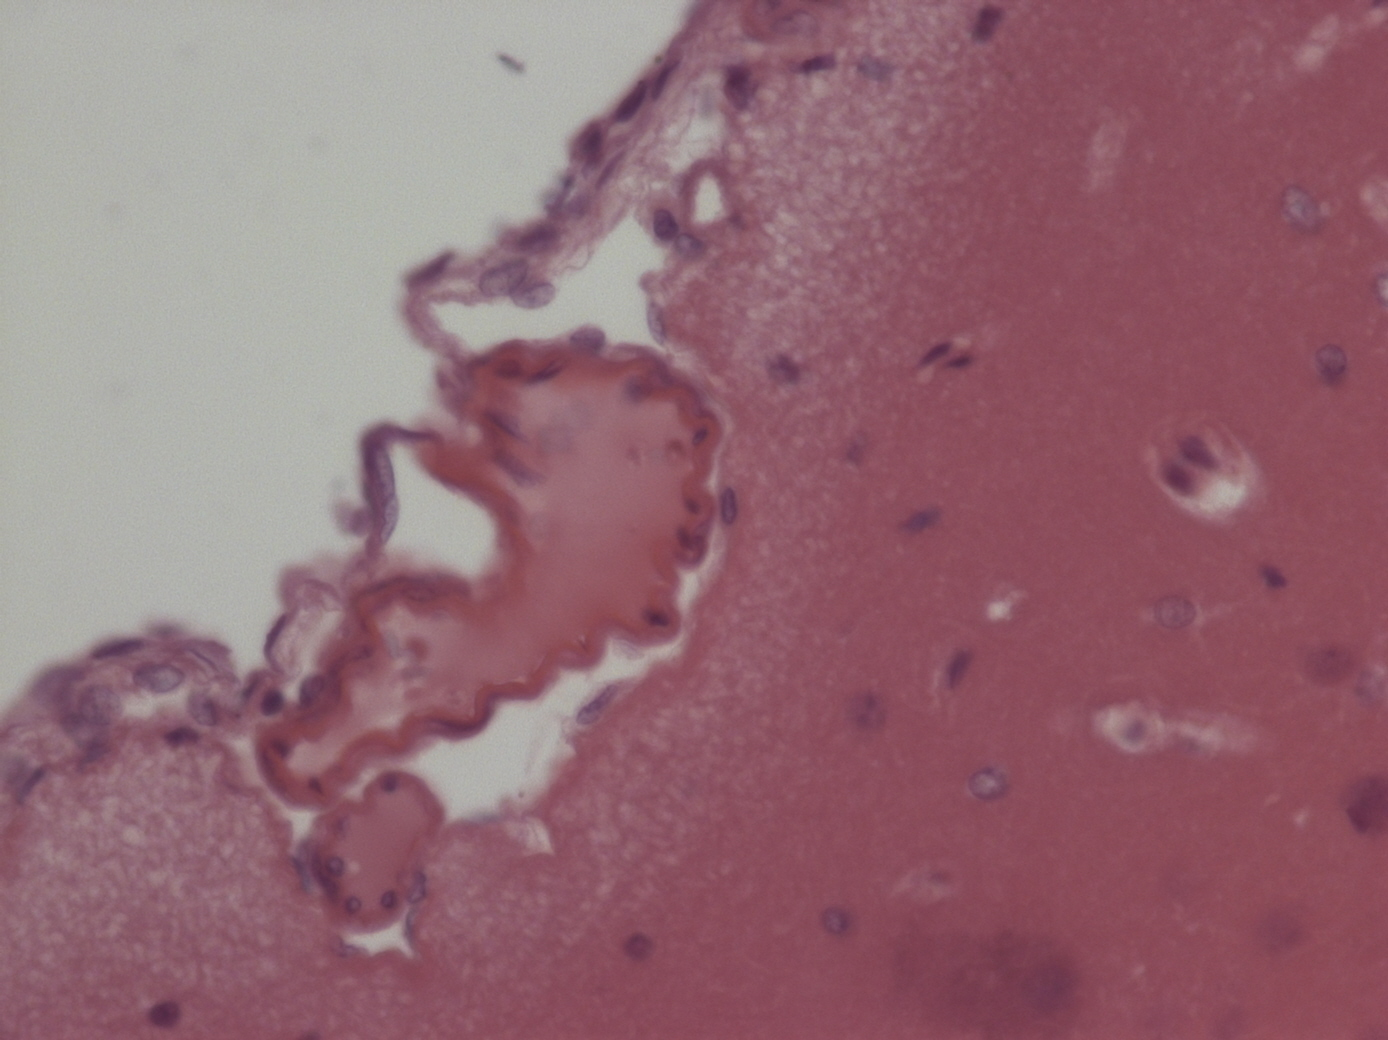
\includegraphics[width=.9\linewidth]{media/5B.jpg}
    }
    \caption{}
    \label{fig:5}
  \end{fullwidth}
\end{figure}

Mice included in the `mixed group', showed some diffuse microhemorrhages, small infiltrations of inflammatory cells, and parasitic sequestration in microvessels (Fig.~\ref{fig:6b}-\ref{fig:6d}) but with no meningeal involvement (Fig.~\ref{fig:6a}) or signs of BBB disruption. These observations suggest that the treatment with SR144528 in these mice slowed down brain damage during the infectious process, as also evidenced by both, the parasitemia curves (Fig.~\ref{fig:3c}) and the neurological phenotypes shown. Thus, our results agree with previous studies where CB\textsubscript{2} knockout mice (Cnr2\textsuperscript{-}/\textsuperscript{-}) exhibit enhanced survival with reduced parasite load in the brain and a diminished BBB disruption \parencite{Alferink2016}. SR144528 treatment in these two mice resulted in an increase in their survival time, reaching day up to day -20 post-infection. However, the compound did not show an antimalarial effect sufficient to eliminate circulating parasites, since parasitemia increased again (Fig.~\ref{fig:3c}) from day -10 onwards, with no neurological manifestations, but to finally cause death by hyperparasitemia and severe anemia.



Due to the low number of animals, the experimental model is inconclusive and, therefore, our initial hypothesis could not be validated. However, these partial results suggest that CM severity could be modulated by the pharmacological blockade of the CB\textsubscript{2} receptors. In addition, other factors might be involved in the further disease evolution. In the first instance, activation of the CB\textsubscript{2} receptor has been associated with a decrease of exacerbated inflammation in several pathologies \parencite{Morales2016, Turcotte2016, Fernández-Ruiz2006, Fernández-Ruiz2015}, in other studies it has been demonstrated that this receptor could also contribute to tissue damage \parencite{Pacher2011}. Different reports have postulated that modulation of the endocannabinoid signaling through the CB\textsubscript{2} receptor, both by agonists and inverse agonists/antagonists, could have a relevant therapeutic potential in a large number of diseases by reducing the inflammatory and chemotactic response and attenuating the endothelial activation and cell adhesion \parencite{Pacher2011}. Regarding CM, in addition to the presumable anti-inflammatory activity that might counteract the exacerbated inflammation of this brain process, inhibition of the CB2 receptor by the SR144528 antagonist could also contribute to the maintenance of the integrity of the BBB. In fact, activation of CB\textsubscript{2} receptor triggers, (among other things)s, MAPK signaling, which has been shown involved in BBB disruption and in vivo neurological symptoms of severe malaria \parencite{Picone2015, Rhee2002}. By blocking CB\textsubscript{2} receptor, the MAPK pathway would be inhibited, thus maintaining BBB integrity.

\begin{figure}
  \begin{fullwidth}
    \raggedleft
    \subcaptionbox{\label{fig:6a}}{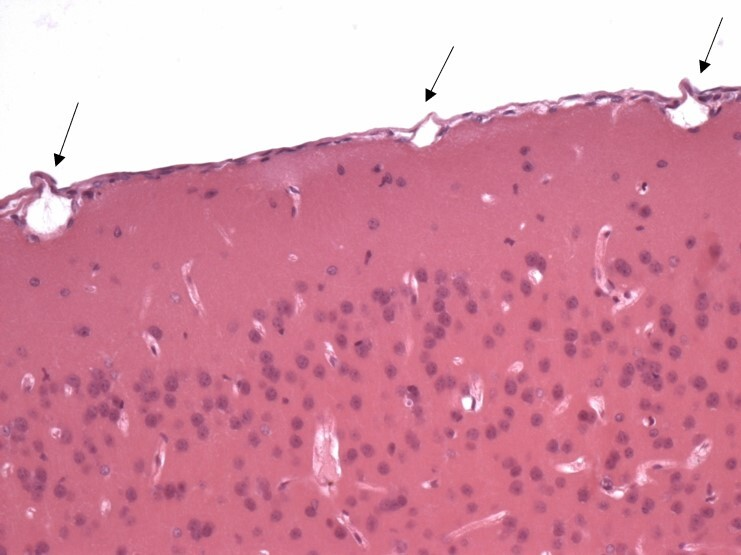
\includegraphics[height=.48\textwidth]{media/6A.jpg}
    }
    \subcaptionbox{\label{fig:6b}}{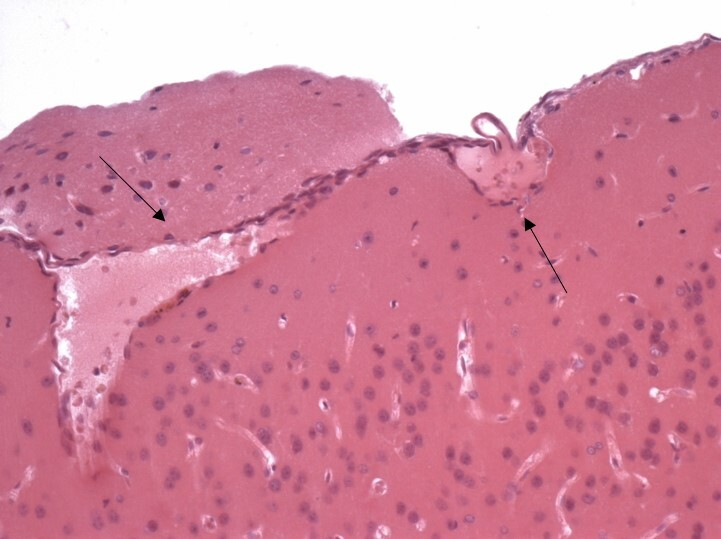
\includegraphics[height=.48\textwidth]{media/6B.jpg}
    }
    \subcaptionbox{\label{fig:6c}}{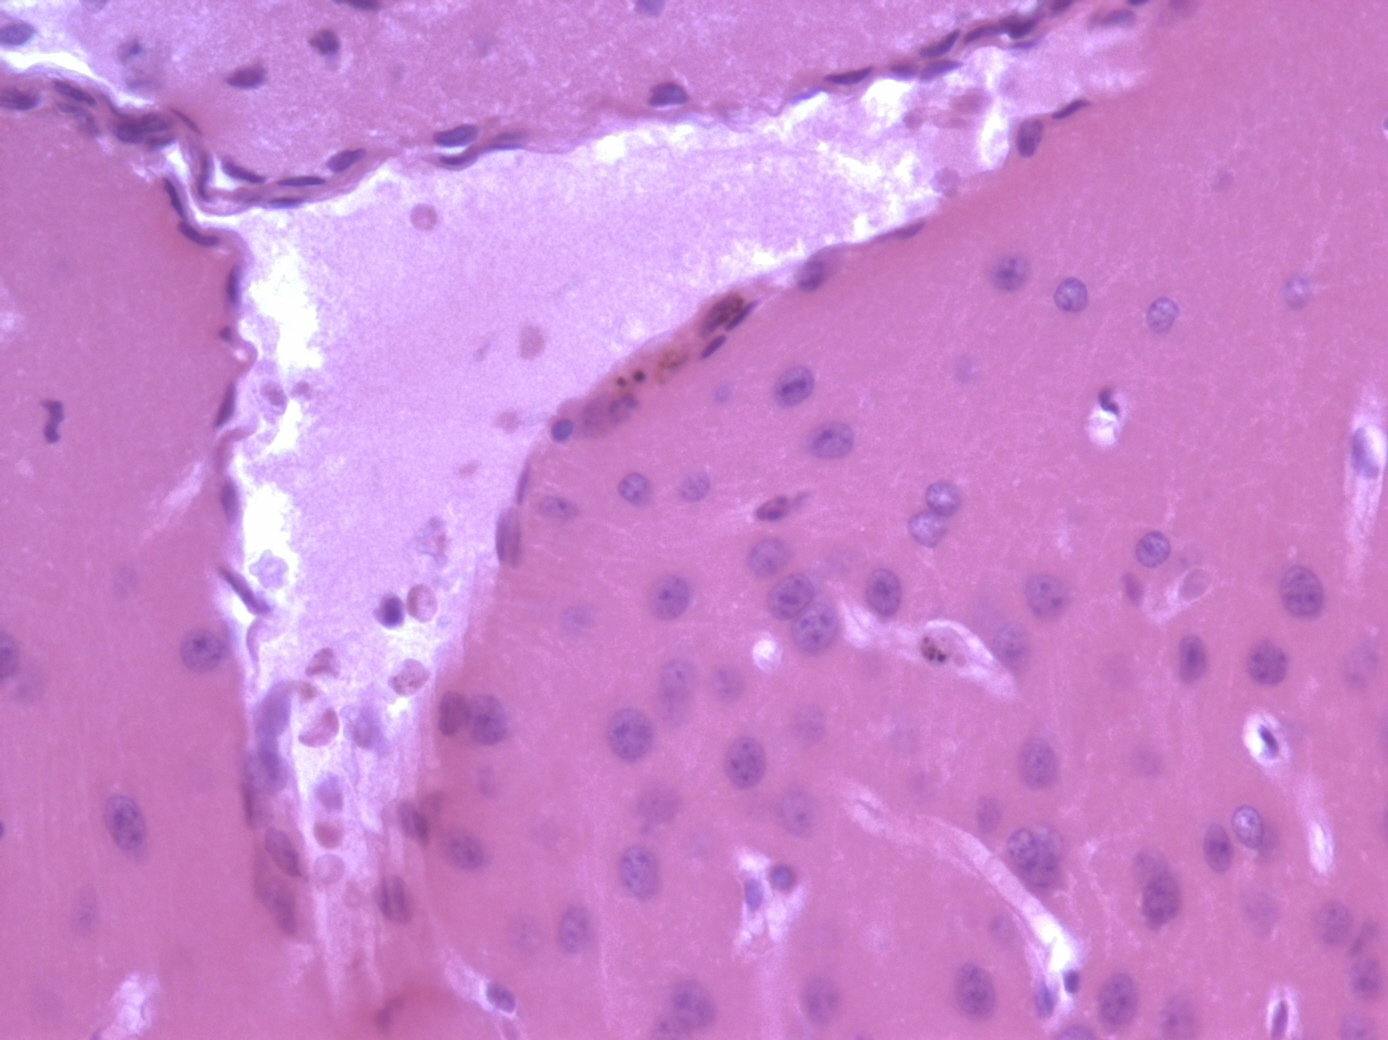
\includegraphics[height=.48\textwidth]{media/6C.jpg}
    }
    \subcaptionbox{\label{fig:6d}}{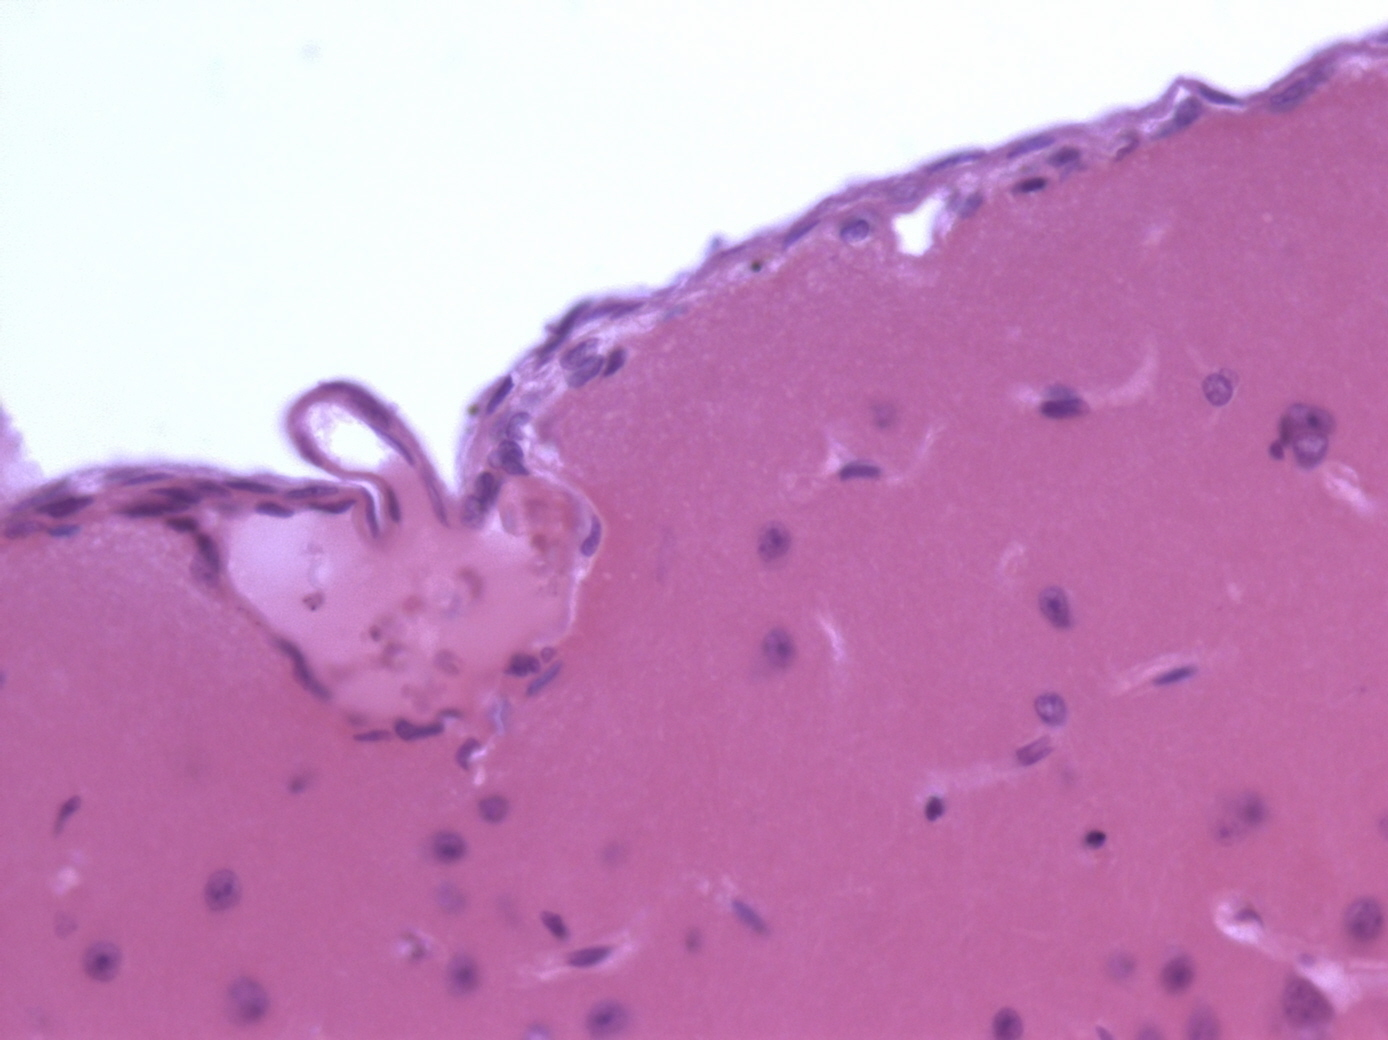
\includegraphics[height=.48\textwidth]{media/6D.jpg}
    }
    \caption{}
    \label{fig:6}
  \end{fullwidth}
\end{figure}


\section{Conclusion}

In this study, we hypothesized modulation and therapeutic potential of CB\textsubscript{2} receptor in the pathophysiology of experimental CM. Through blockade by SR144528, (a CB\textsubscript{2} receptor selective antagonist), in an in vivo murine model of CM, 30\% of the treated mice showed partial recovery of CM symptoms with 20\% increased survival while, but finally succumbing to hyperparasitaemia and severe anemia. Although other factors seem to be involved in controlling the infection and our results are inconclusive, the present observations provide valuable experimental information for the development of alternative treatment regimens for CM by combining classic antimalarial drugs and neuroprotective compounds targeting CB\textsubscript{2}. Thus, we suggest that SR144528 could be used as an adjuvant in the treatment of CM for a rescue therapy that could prevent or eliminate neurological sequelae in individuals who survive the infection. Further experimental pharmacological studies would be interesting to elucidate optimal candidates.

\nocite{*}
\printbibliography

% \emph{Journal of Biological Chemistry}, \emph{291}(37), 19517--19531. https://doi.org/10.1074/jbc.M116.746594

% Bartoloni, A., \& Zammarchi, L. (2012). Clinical aspects of uncomplicated and severe malaria. \emph{Mediterranean Journal of Hematology and Infectious Diseases}, \emph{4}(1), e2012026. https://doi.org/10.4084/MJHID.2012.026

% Brian De Souza, J., Hafalla, J. C. R., Riley, E. M., \& Couper, K. N. (2010). Cerebral malaria: Why experimental murine models are required to understand the pathogenesis of disease. \emph{Parasitology}. https://doi.org/10.1017/S0031182009991715

% Campos, A. C., Brant, F., Miranda, A. S., Machado, F. S., \& Teixeira, A. L. (2015). Cannabidiol increases survival and promotes rescue of cognitive function in a murine model of cerebral malaria. \emph{Neuroscience}, \emph{289}, 166--180. https://doi.org/10.1016/j.neuroscience.2014.12.051

% Combes, V., Coltel, N., Faille, D., Wassmer, S. C., \& Grau, G. E. (2006). Cerebral malaria: role of microparticles and platelets in alterations of the blood-brain barrier. \emph{International Journal for Parasitology}, \emph{36}(5), 541--546. https://doi.org/10.1016/j.ijpara.2006.02.005

% Cumella, J., Hernández-Folgado, L., Girón, R., Sánchez, E., Morales, P., Hurst, D. P., … Jagerovic, N. (2012). Chromenopyrazoles: Non-psychoactive and Selective CB 1 Cannabinoid Agonists with Peripheral Antinociceptive Properties. \emph{ChemMedChem}, \emph{7}(3), 452--463. https://doi.org/10.1002/cmdc.201100568

% Deiana, V., Gómez-Cañas, M., Pazos, M. R., Fernández-Ruiz, J., Asproni, B., Cichero, E., … Pinna, G. A. (2016). Tricyclic pyrazoles. Part 8. Synthesis, biological evaluation and modelling of tricyclic pyrazole carboxamides as potential CB2 receptor ligands with antagonist/inverse agonist properties. \emph{European Journal of Medicinal Chemistry}, \emph{112}, 66--80. https://doi.org/10.1016/J.EJMECH.2016.02.005

% Fernández-Ruiz, J., Romero, J., \& Ramos, J. A. (2015). Endocannabinoids and neurodegenerative disorders: Parkinson's disease, huntington's chorea, alzheimer's disease, and others. In \emph{Endocannabinoids} (Vol. 231, pp. 233--259). https://doi.org/10.1007/978-3-319-20825-1\_8

% Fernández-Ruiz, J., Romero, J., Velasco, G., Tolón, R. M., Ramos, J., \& Guzmán, M. (2006). Cannabinoid CB 2 receptor : a new target for controlling neural cell survival ?, \emph{28}(1). https://doi.org/10.1016/j.tips.2006.11.001

% Fogaça, M. V., Galve-Roperh, I., Guimarães, F. S., \& Campos, A. C. (2013). Cannabinoids, Neurogenesis and Antidepressant Drugs: Is there a Link? \emph{Current Neuropharmacology}, \emph{11}(3), 263--275. https://doi.org/10.2174/1570159X11311030003

% Grau, G. E., Fajardo, L. F., Piguet, P.-F., Allet, B., Lambert, P.-H., \& Vassalli, P. (1987). Tumor necrosis factor (cachetin) as an essential mediator in murine cerebral malaria. \emph{Science}, \emph{237}(4819), 1210--1213.

% Hunt, N. H., Golenser, J., Chan-Ling, T., Parekh, S., Rae, C., Potter, S., … Ball, H. J. (2006). Immunopathogenesis of cerebral malaria. \emph{International Journal for Parasitology}, \emph{36}(5), 569--582. https://doi.org/10.1016/J.IJPARA.2006.02.016

% Hunt, N. H., \& Grau, G. E. (2003). Cytokines: accelerators and brakes in the pathogenesis of cerebral malaria. \emph{Trends in Immunology}, \emph{24}(9), 491--499. https://doi.org/10.1016/S1471-4906(03)00229-1

% Linares, M., Marín-García, P., Pérez-Benavente, S., Sánchez-Nogueiro, J., Puyet, A., Bautista, J. M., \& Diez, A. (2013). Brain-derived neurotrophic factor and the course of experimental cerebral malaria. \emph{Brain Research}, \emph{1490}, 210--224. https://doi.org/10.1016/j.brainres.2012.10.040

% Lou, J., Lucas, R., \& Grau, G. E. (2001). Pathogenesis of Cerebral Malaria: Recent Experimental Data and Possible Applications for Humans, \emph{14}(4), 810--820. https://doi.org/10.1128/CMR.14.4.810--820.2001

% Marín-García, P., Sánchez-Nogueiro, J., Diez, A., León-Otegui, M., Linares, M., García-Palencia, P., … Miras-Portugal, M. T. (2009). Altered Nucleotide Receptor Expression in a Murine Model of Cerebral Malaria. \emph{The Journal of Infectious Diseases}, \emph{200}(8), 1279--1288. https://doi.org/10.1086/605896

% Mariotti, R., \& Bertini, G. (2011). Neuroinflammation and brain infections: Historical context and current perspectives. \emph{Brain Research Reviews}, \emph{66}(1--2), 152--173. https://doi.org/10.1016/J.BRAINRESREV.2010.09.008

% Martínez-pinilla, E., Varani, K., Reyes-resina, I., Angelats, E., Vincenzi, F., Ferreiro-vera, C., … Martínez-pinilla, E. (2017). Binding and Signaling Studies Disclose a Potential Allosteric Site for Cannabidiol in Cannabinoid CB 2 Receptors, \emph{8}(October), 1--10. https://doi.org/10.3389/fphar.2017.00744

% Martinez, G., Linares, M., Marin-Garcia, P., Benavente, S. P., Puyet, A., Bautista, J., \& Diez, A. (2013). \emph{Standardization of a cerebral malaria murine model in clinical stages for antimalarial and rescue therapies evaluation}. \emph{Anales de la Real Academia Nacional de Farmacia} (Vol. 79).

% Medana, I. M., \& Turner, G. D. H. (2006). Human cerebral malaria and the blood--brain barrier. \emph{International Journal for Parasitology}, \emph{36}(5), 555--568. https://doi.org/10.1016/J.IJPARA.2006.02.004

% Morales, P., Gómez-Cañas, M., Navarro, G., Hurst, D. P., Carrillo-Salinas, F. J., Lagartera, L., … Jagerovic, N. (2016). Chromenopyrazole, a Versatile Cannabinoid Scaffold with in Vivo Activity in a Model of Multiple Sclerosis. \emph{Journal of Medicinal Chemistry}, \emph{59}(14), 6753--6771. https://doi.org/10.1021/acs.jmedchem.6b00397

% Pacher, P., \& Mechoulam, R. (2011). Is lipid signaling through cannabinoid 2 receptors part of a protective system? \emph{Progress in Lipid Research}, \emph{50}(2), 193--211. https://doi.org/10.1016/j.plipres.2011.01.001

% Pazos, M. R., Cinquina, V., Gómez, A., Layunta, R., Santos, M., Fernández-Ruiz, J., \& Martínez-Orgado, J. (2012). Cannabidiol administration after hypoxia--ischemia to newborn rats reduces long-term brain injury and restores neurobehavioral function. \emph{Neuropharmacology}, \emph{63}(5), 776--783. https://doi.org/10.1016/j.neuropharm.2012.05.034

% Picone, R. P., \& Kendall, D. A. (2015). Minireview: From the Bench, Toward the Clinic: Therapeutic Opportunities for Cannabinoid Receptor Modulation. \emph{Molecular Endocrinology}, \emph{29}(6), 801--813. https://doi.org/10.1210/me.2015-1062

% Portier, M., Rinaldi-Carmona, M., Pecceu, F., Combes, T., Poinoit-Chazel, C., Calandra, B., … Casellas, P. (1999). SR 144528, an antagonist for the peripheral cannabinoid receptor that behaves as an inverse agonist - PubMed. \emph{Journal of Pharmacology and Experimental Therapeutics}, \emph{288}(2), 582--589.

% Rhee, M.-H., \& Sang-Keun, K. (2002). SR144528 as Inverse Agonist of CB2 Cannabinoid Receptor. \emph{Journal of Veterinary Science}, \emph{3}(3), 179--184.

% Rinaldi-Carmona, M., Barth, F., Héaulme, M., Shire, D., Calandra, B., Congy, C., … Le Fur, G. (1994). SR141716A, a potent and selective antagonist of the brain cannabinoid receptor. \emph{FEBS Letters}, \emph{350}(2--3), 240--244. https://doi.org/10.1016/0014-5793(94)00773-X

% Rinaldi-Carmona, M., Barth, F., Millan, J., Derocq, J. M., Casellas, P., Congy, C., … Le Fur, G. (1998). SR 144528, the first potent and selective antagonist of the CB2 cannabinoid receptor. \emph{Journal of Pharmacology and Experimental Therapeutics}, \emph{284}(2), 644--650.

% Ross, M. H., Pawlina, W., \& Negrete, J. H. (2007). \emph{Histología : texto y atlas color con biología celular y molecular}. Médica Panamericana.

% Turcotte, C., Blanchet, M.-R., Laviolette, M., \& Flamand, N. (2016). The CB2 receptor and its role as a regulator of inflammation. \emph{Cellular and Molecular Life Sciences : CMLS}, \emph{73}(23), 4449--4470. https://doi.org/10.1007/s00018-016-2300-4









\end{document}
